\documentclass[runningheads]{llncs}
\usepackage{graphicx}
\usepackage{float}
\usepackage{caption}
\usepackage{url}
\usepackage{subfigure}
\usepackage{listings}
\usepackage{xcolor}

\definecolor{codegreen}{rgb}{0,0.6,0}
\definecolor{codegray}{rgb}{0.5,0.5,0.5}
\definecolor{codepurple}{rgb}{0.58,0,0.82}
\definecolor{backcolour}{rgb}{0.95,0.95,0.92}
 
\lstdefinestyle{mystyle}{
    backgroundcolor=\color{backcolour},   
    commentstyle=\color{codegreen},
    keywordstyle=\color{magenta},
    numberstyle=\tiny\color{codegray},
    stringstyle=\color{codepurple},
    basicstyle=\ttfamily\footnotesize,
    breakatwhitespace=false,         
    breaklines=true,                 
    captionpos=b,                    
    keepspaces=true,                 
    numbers=left,                    
    numbersep=5pt,                  
    showspaces=false,                
    showstringspaces=false,
    showtabs=false,                  
    tabsize=2
}
 
\lstset{style=mystyle}



\title{The implementation of a browser-based source code navigator and its cloud solution}
\author{Tong Zhou 180275186}
\institute{School of Computing, Newcastle University \\ Newcastle upon Tyne, NE1 7RU}

\begin{document}

%=============================
%===     Title Page   ========
%=============================

\begin{titlepage}
	\begin{center}
	
	
\includegraphics[width=0.65\textwidth]{pic/newcastle-uni-logo.png}\\[3cm]
	
	\textbf{\LARGE The implementation of a browser-based source code navigator and its cloud solution}
	
	~\\
	~\\
	
	\large Submitted by
	
	~\\
	
	\Large Tong \textsc{Zhou}
	
	dns.t.zhou@gmail.com
	
	~\\
	~\\
	
	% Author and supervisor
	\begin{minipage}{0.4\textwidth}
	\begin{flushleft} \large
	\emph{Industrial Director:}\\
	Jonathan \textsc{Halliday}
	\end{flushleft}
	\end{minipage}
	\begin{minipage}{0.4\textwidth}
	\begin{flushright} \large
	\emph{Academic Supervisor:} \\
	Dr.~Paul \textsc{Ezhilchelvan}
	\end{flushright}
	\end{minipage}
	
	~\\
	~\\
	~\\
	
	\textit{Submitted in partial requirements for the degree of
	Master of Science in Cloud Computing}
	
	~\\
	~\\
	
	\Large School of Computing
	
	\Large Newcastle University

	~\\

	\large {August 2019}
	
	\end{center}
	\end{titlepage}

\newpage
\pagenumbering{roman}
\setcounter{page}{2}
%=============================
%=== Abstract ============
%=============================
\section*{Abstract}
\addcontentsline{toc}{section}{Abstract}
An integrated development environment (IDE) is a software application that provides comprehensive facilities to computer programmers for software development\cite{Integrated_development_environment}, but on certain occasions, developers want to browse all java files within an entire jar file.

This dissertation is mainly about the design and implements of a kind of web-based source code navigator for Java, called Online Java Navigator, which provides an online user interface for all developers to browse specific repositories of java source code. Different users can access a general server that uses a unified storage system to look up all relevant information required to resolve the navigation result. With this browser-based source code navigation system, users can view every Java file as an online web page, and click any validated type name within the page, then the system will direct them to the right target java type that is quoted by current scope.

To provide service to users from all over the world, a good cloud structure is pretty crucial during both deployment stage and development stage. There are different kind of solutions to choose from, and all these solutions have their advantages and disadvantages, thus an evaluation of these solutions was conducted during this project.

\section*{Declaration}
\addcontentsline{toc}{section}{Declaration}

I declare that this dissertation represents my own work except where otherwise explicitly stated.

\newpage
%=============================
%=== Acknowledgements ============
%=============================
\section*{Acknowledgements}
\addcontentsline{toc}{section}{Acknowledgements}

Firstly, I would like to express my thanks to Mr Jonathan Halliday and Dr Paul Ezhilchelvan for their help, advice and patient guidance during this project. I would also like to expand my gratitude to all those who have directly and indirectly guided me in writing this dissertation.

Also, I would like to express my gratitude to my lecturers during the entire MSc programme: Dr Paul Ezhilchelvan, Dr Ellis Solaiman, Dr Stephen McGough,  Dr Nigel Thomas,  Professor Raj Ranjan,  Dr Yu Guan, Dr Paolo Missier. There were so much useful knowledge and information I achieved from those lectures, which benefits me a lot both academically and practically.

This project was so much different from any of my previous project because this was an industrial student project which requires for both academic knowledge and engineering practice, and this project benefited me a lot during the past four months.

Finally, I would like to thank the Newcastle University and Red Hat Ltd in general, for all kinds of support from academic materials to facility resources during my project.


\newpage
\tableofcontents

\newpage
\pagenumbering{arabic}
\setcounter{page}{1}
%=============================
%=== 1 Introduction ============
%=============================
\section{Introduction}

This dissertation is mainly about the design and implements of a web-based source code navigator for Java, called \textbf{Online Java Navigator}\cite{ojn-Repository}, which provides an online user interface for all developers to browse specific repositories of java source code.

\begin{figure}[H]
	\centering
	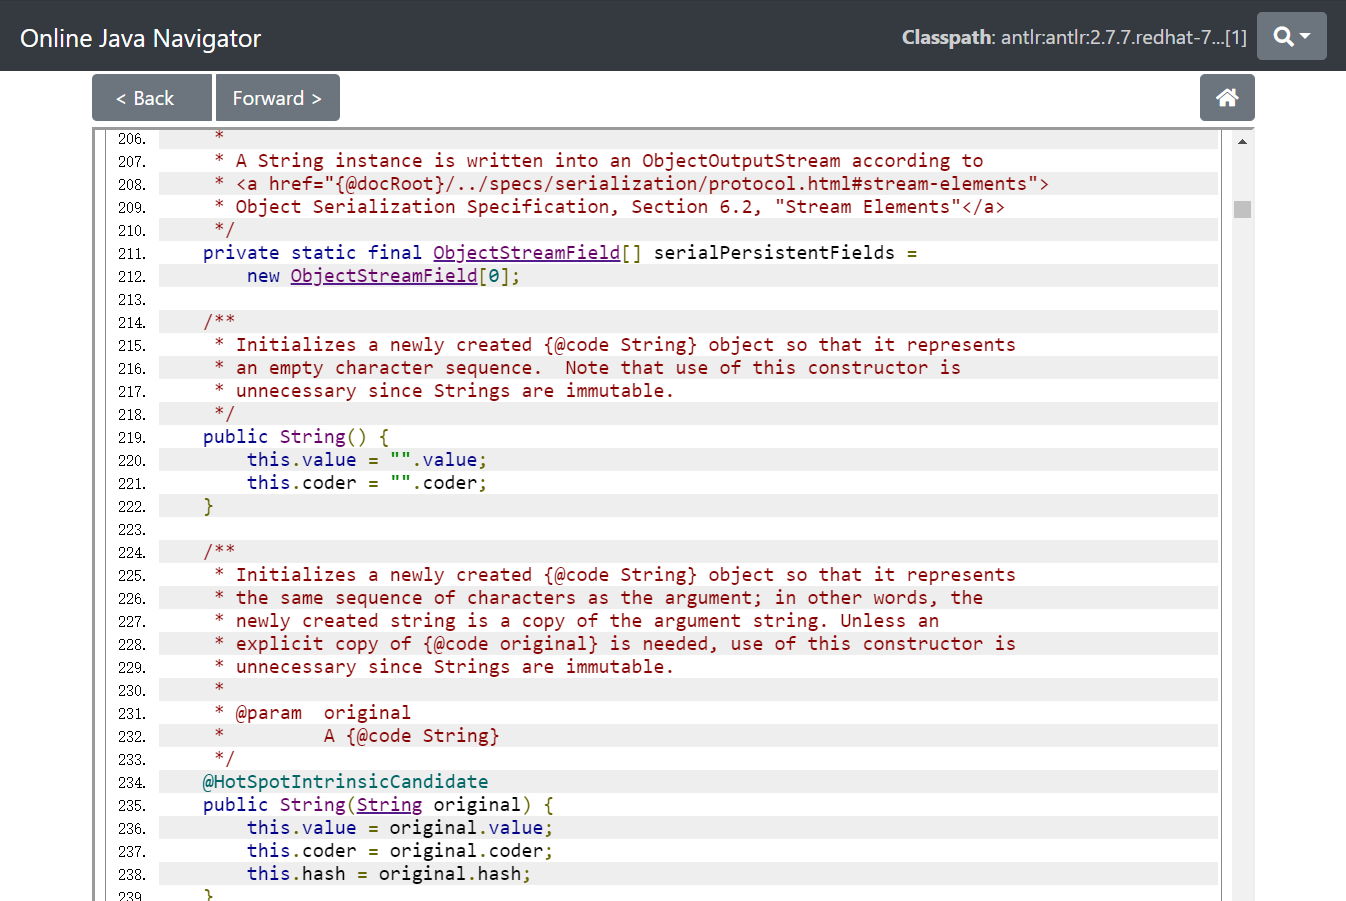
\includegraphics[width=12cm]{pic/OJNWebPage.png}
	\caption{Product User Interface}
	\label{product user interface}
\end{figure}

With this system, users can view every java file as an online web page, and click any validated type name within the page, then the system will direct them to the right target java type that is quoted by current scope.
The system support user-customised classpath, which means the user can define the boundaries of browsing and navigate only within a specific scope of source code. Also, all java codes are displayed with syntax highlighting, so that users would have a better user experience while reading those codes.

The system uses a non-container solution, which means it is different from the online IDE system. An online IDE uses container technology to create an individual container for each user instance so that they can browse, run and debug code remotely, it does help to build a robust environment for developer to use online but at the cost of a lot of resources consumed to provide service to developers from all over the world. Instead, a non-container solution uses a universal server group for any access from the internet and provide service with low cost and high efficiency.
The product is deployed on AWS public cloud with CDN\cite{Content_delivery_network} and BLOB\cite{Binary_large_object} storage system, which means it can provide service to users from all over the world with high availability and low latency.

You can access the demo environment of this project via this link: 

http://bit.ly/2T5ODrx


%=============================
%===      2	Background      ====
%=============================
\section{Background}

An integrated development environment (IDE) is a software application that provides comprehensive facilities to computer programmers for software development\cite{Ide_introduction}. A handy feature provided by IDE is the ability to navigate between different files so that they can conveniently navigate the Types that used in any part of codes. Currently, there are a lot of IDE that provides useful functions like that, but sometimes developers may want to browse code online as a document. For single file cases, this is sometimes possible; for example, GitHub\cite{GitHub} provides an online webpage for every file in the repository, user can easily browse and edit the code. 

On certain occasions, developers want to browse all java files within an entire jar file, because now software products are becoming more and more complicated, developers are trended to implement some open-source project into their product to boost their development, and these open-source products are usually packed as jar files. Within these jar files, there are a lot of java files which have internal quotes with each other, just like when you import specific java class and use it in another java class. Because of this domestic relationship between different java files, it is especially useful if developers can browse all related open-source code online with navigation between different java files, just like what a local IDE can provide to users.


\subsection{Current solutions}
There are some existing solutions and products on the market that provide these features, which can be concluded as two types of solutions:

\subsubsection{Container-based solutions: Gitpod\cite{Gitpod}, SourceGraph\cite{SourceGraph}}

These two products similarly provide an individual container to every user instances. Within the container, the system automatically builds a java development environment and integrate a front-end user interface to interact with users. When the user loads any specific project, it passes the code to the container, then compiles, build and debug it in realtime.

\begin{figure}[H]
	\centering
	\begin{minipage}[t]{0.48\textwidth}
	\centering
	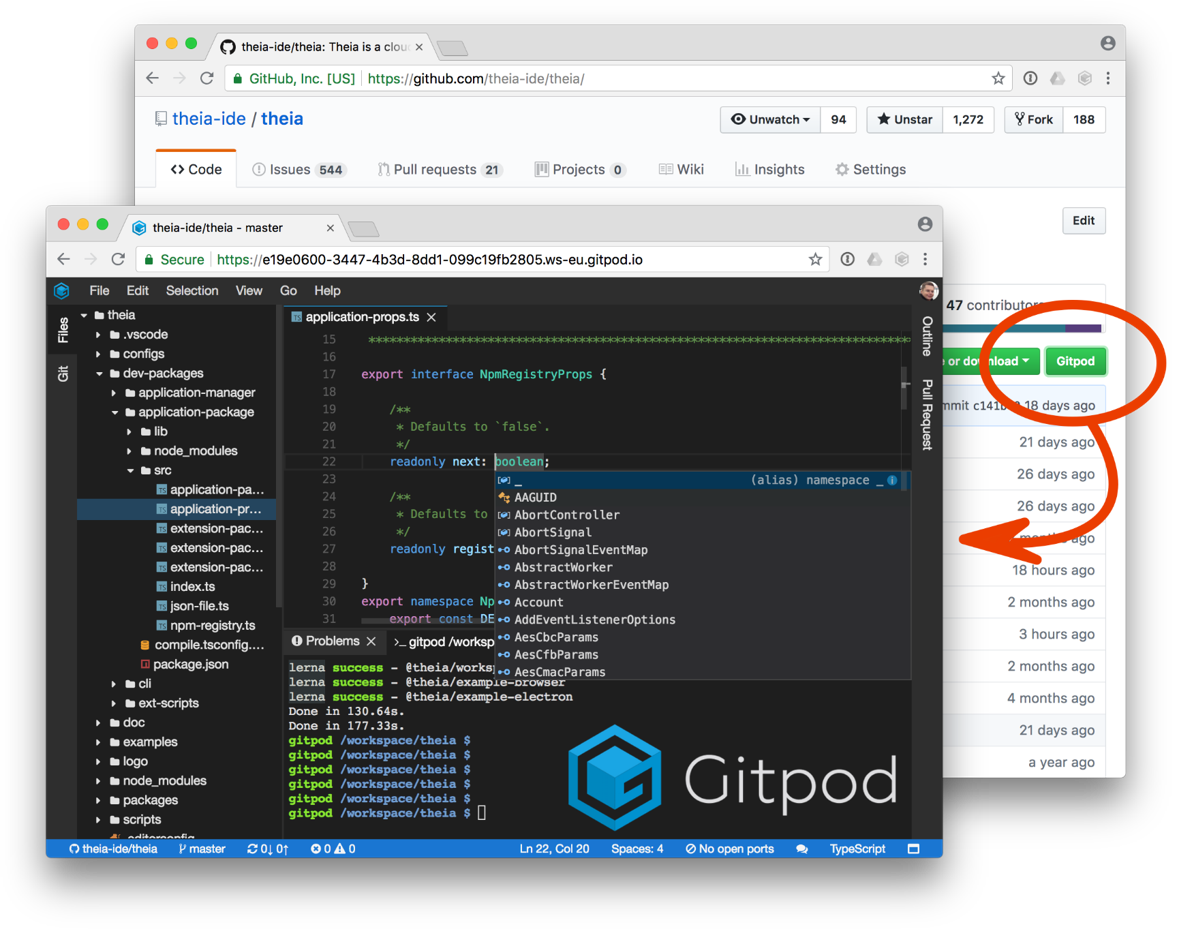
\includegraphics[width=5.8cm]{pic/gitpod.png}
	\caption{Gitpod}
	\end{minipage}
	\begin{minipage}[t]{0.48\textwidth}
	\centering
	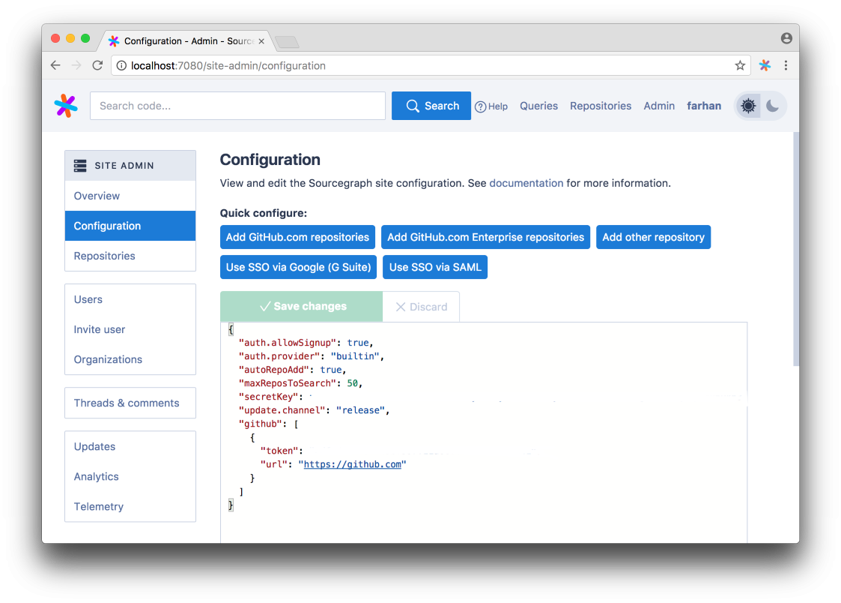
\includegraphics[width=5.8cm]{pic/sourcegraph.png}
	\caption{Sourcegraph}
	\end{minipage}
\end{figure}

This kind of solution can provide the most potent online IDE to users, making it almost the same as an offline development environment. But on the other hand, it cost a lot of resources to support this type of solution, because to use the system, every user will need a complete runtime environment individually. And in terms of open-source code, the user may merely want to browse and look up the source code repository to learn how to implement that product or figure out the root cause of some defect occurred during their implementation. For this kind of user requirement, it would be to luxury to provide an entire IDE environment to users, and that would cost too much to provide service to tremendous of users from all over the world.


\subsubsection{Non-container solution: zGrepCode\cite{zgrepcode}}
This product is almost the ideal solution for our requirement. It firstly analysis the source code and index them, then provide online access for users to browse and navigate among different java files. It does not provide any customised container to users; instead, it uses a general server to resolve all links by querying the index generated previously.

\begin{figure}[H]
	\centering
	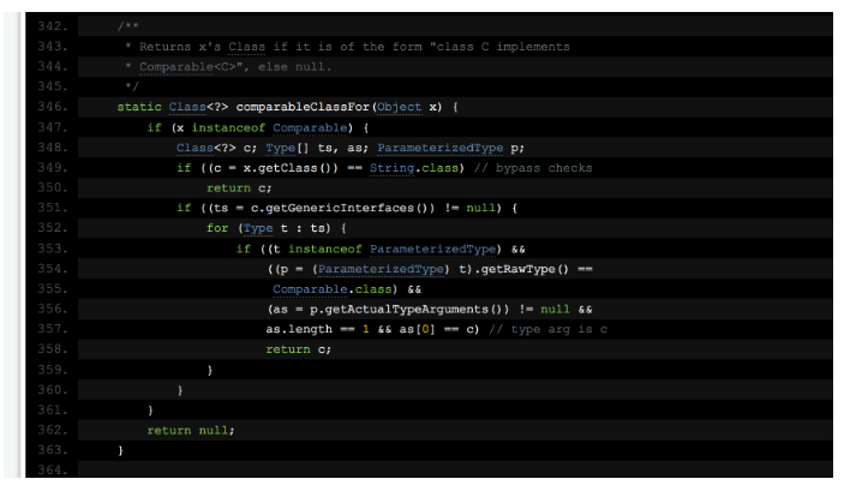
\includegraphics[width=8cm]{pic/zGrepCode.png}
	\caption{zGrepCode}
	\label{zGrepCode}
\end{figure}

But zGrepCode does not provide users with the ability to customise their own configurations and preferences. For example, user can not nominate some specific version of JDK or any other open-source repository with specified version id, which makes it difficult for users to build their own scope of the repository. Developers may want a repository with java 8 and JUnit 3, if this scope is not pre-designed by zGrepCode, users will have no way to config it by them self.

Even worse, this product has been out of service for a few months, and there is no indication whether it will be available in the future.

\subsection{Compilation and execution of Java program}
Other languages like Python and JavaScript have a lot of existing tools to use. How ever, there are not many tools providing a similar function for Java, because it is more challenging to implement a navigation system for java code, because of the complexity of its compilation and execution process.

\begin{figure}[H]
	\centering
	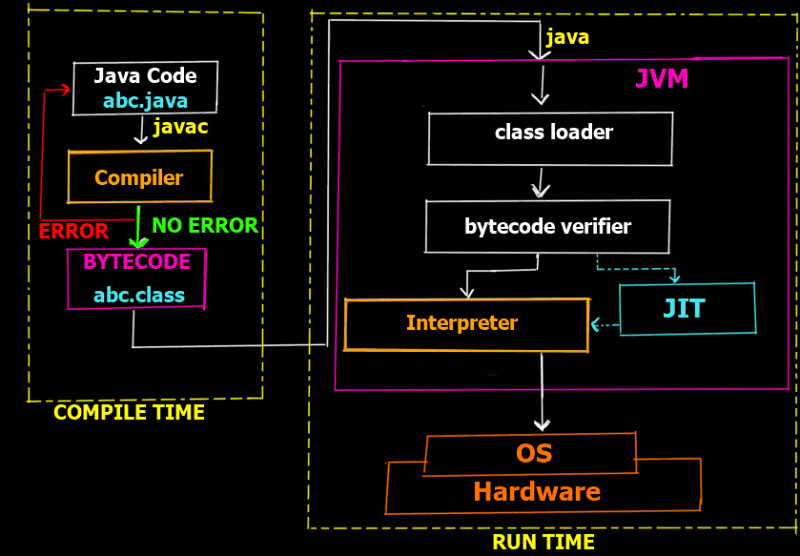
\includegraphics[width=12cm]{pic/java-execution-process.png}
	\caption{Execution process of Java program in detail\cite{java-execution-process}}
	\label{Execution process of Java program in detail}
\end{figure}

There are two processes working individually, which is the compiled time and run time. In each process, the original java code is processed separately with different rules, and the behaviour of type navigation that presented to the user is a combination of the result from both processes. If we want to implement a source code navigation system without compile time and run time, a general rule for navigation is required to build this system, but currently, there is no relevant research that purposed such kind of general rules.

\subsection{General requirement}
Base on the research mentioned above, this project was proposed by Red Hat, which aimed to develop a browser-based source code navigation system for open-source developers and their customers. This navigation system should meet the following requirements:

\begin{enumerate}
	\item User should be available to browse all Java codes from the repositories online.
	\item The system should allow users to config customised classpath which defines some specific versions of dependencies to involve in the current scope of code. 
	\item The code displayed online should be syntax highlighted so that the user can easily browse the code on the webpage.
	\item This product should be available to provide service to multiple users at the same time and at the same time, cost as less computing resource as possible.
	\item The code should be efficient enough to: 
	\begin{enumerate}
		\item Provide cost-efficient operation of the bulk rendering component, with a time budget of 10ms per input source java file on a single CPU core.
		\item Provide responsive user interaction for the link resolution, with a time budget of 50ms for returning a response, excluding network RTT, given a single concurrent user on a single CPU core with 2GB memory.
	\end{enumerate}
\end{enumerate}


%=============================
%===3 Comparative Research====
%=============================
\section{Comparative Research}

There are a lot of different open-sourced projects that can help develop a browser-based source code navigation system, so before designing this project, several products were evaluated, and a general comparison can be found as follow.

\subsection{Java Parsing}

Without the process of a specific parser, the raw java file is just a combination of characters, so firstly it is essential to find an appropriate solution to parse the source code. 

A parser is usually composed of two parts: a lexer, also known as scanner or tokenizer, and the proper parser. Not all parsers adopt this two-steps schema: some parsers do not depend on a lexer. They are called scannerless parsers.\cite{parsing-in-java}

\begin{itemize}
	\item \textbf{Lexer + Parser solution:} AnnoFlex\cite{AnnoFlex} + Antlr\cite{Antlr}

	AnnoFlex Bases on annotation (own JavaDoc labels) to produces the matching tokens, and then use Antlr to generate an AST.

	This solution is a little bit complex, and the improper JavaDoc labels will also cause syntax warning from syntax highlight tool and IDE.

	\item \textbf{CFG(Context-free grammars) solution:} Antlr\cite{Antlr}

	This kind of solution is widely used to generate parsers. You can define your own grammar and use it to create a parser that works for it. It is a basic low-level tool, but for our project, the language is predefined for Java only, so there is no need to spend a lot of effort on creating our own parser.

	\item \textbf{PEG(Parsing Expression Grammar) solution:} JavaParser\cite{JavaParser}

	Java Parser is A well-organised parser derived from JavaCC. It supports all versions of java from 1 to 12, and it also supports lexical preservation and pretty printing. It is also Eligible to use with JavaSymbolSolver, which can boost up our project to save a lot of effort to implement such kind of functions.
\end{itemize}
Obviously, for this project, the JavaParser would be the best solution to implement our own parsing functions.

\subsection{Syntax Highlight}
In order to prettify the code with syntax highlight and make it more similar to a local IDE, this project requires a tool to provide syntax highlight. There are three products been evaluated during this project, which is Syntax Highlighter\cite{syntaxhighlighter}, Code Mirror\cite{codemirror}, Code Prettify\cite{code-prettify}.

\begin{figure}[H]
	\centering
	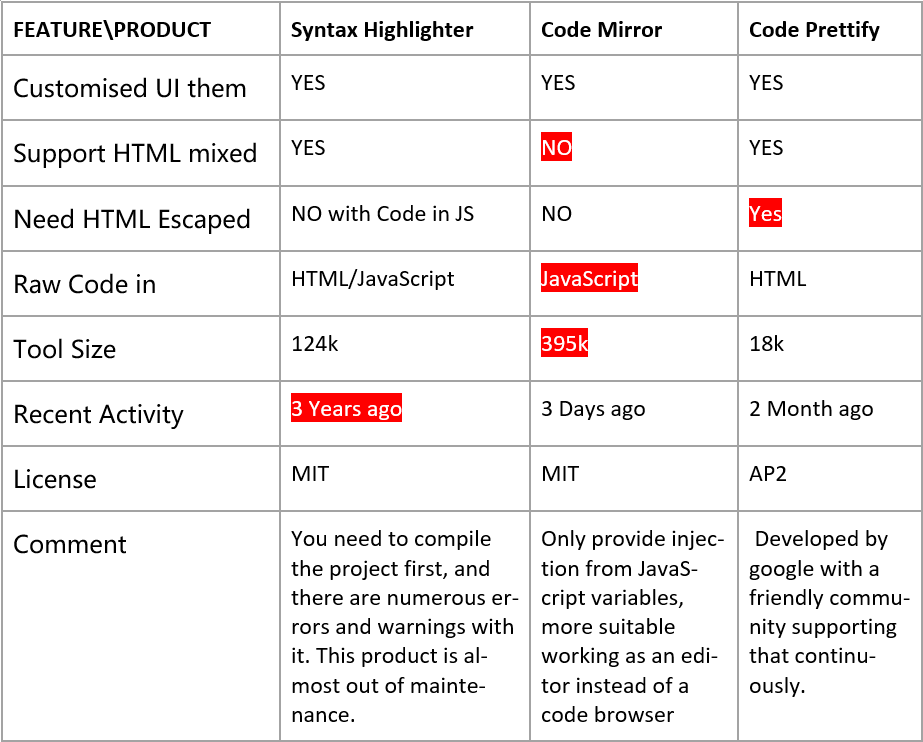
\includegraphics[width=12cm]{pic/highlighter-metrix.png}
	\caption{Metrix of different syntax highlighting tools}
	\label{Metrix of different syntax highlighting tools}
\end{figure}

After the comparison between all three products, it is more appropriate to integrate Code Prettify into our project to provide a syntax highlight feature.

\subsection{Front-end Framework}
This navigation system provides a browser-based user interface for the developer to access, at the same time send, receive and process information during the entire resolving stage. Thus, a front-end framework is especially important.

\begin{figure}[H]
	\centering
	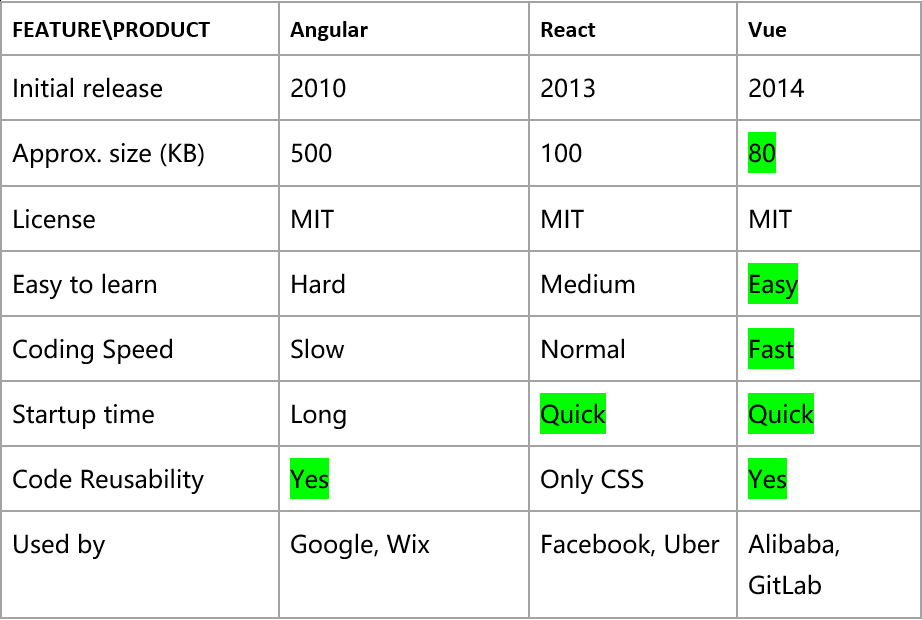
\includegraphics[width=12cm]{pic/front-end-metrix.png}
	\caption{Metrix of front-end frameworks}
	\label{Metrix of front-end frameworks}
\end{figure}

In terms of this project, the front-end logic is not complicated at all, so a light front-end framework like Vue.js would be the best choice. 

%=============================
%===4 High-level Architecture====
%=============================
\section{High-level Architecture}

According to what required in paragraph 2.3, this system should adopt a non-container solution to provide service to as many users as possible. 

\begin{figure}[H]
	\centering
	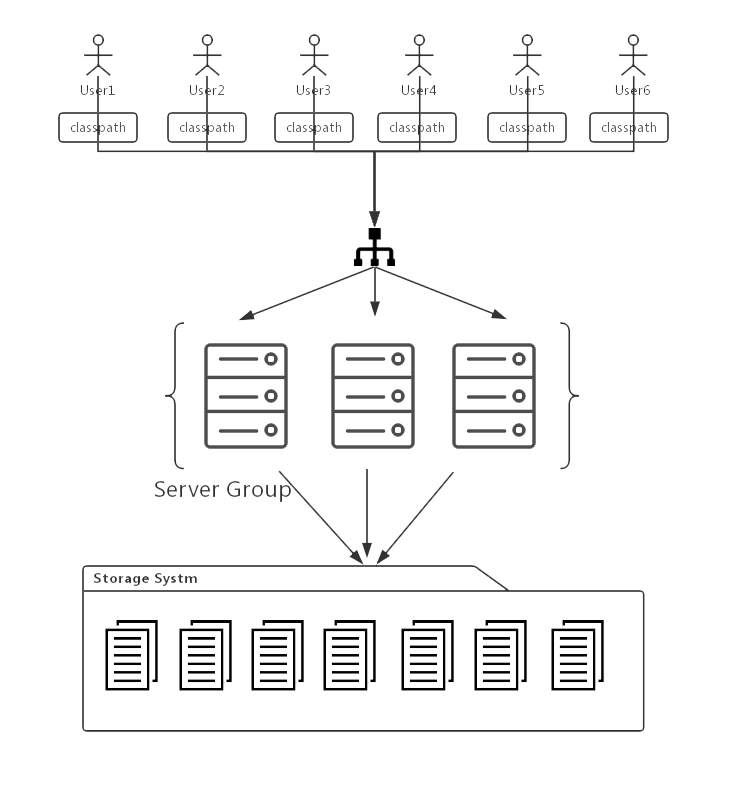
\includegraphics[width=9cm]{pic/high-level-diagram.png}
	\caption{High level user access}
	\label{High level user access}
\end{figure}

But with a non-container solution, it is impossible to use JVM to resolve the symbol in realtime. Instead, different users should be able to access a general server(or server group) that uses a unified storage system to look up all relevant information required to resolve the navigation result(see Fig. 8). Thus, the navigator is designed as a two-stage system:

\begin{itemize}
	\item \textbf{Stage1: Analysis Process}

	In this stage, the system scans all java codes in the .jar files within the repository, converts them into Html document. Every Java types are wrapped with hyperlink tags so that all types(classes, interfaces, annotations) within this Html file can be easily recognised by the user, and the user can click the hyperlink to request for navigation to redirect to the definition of this specific type.

	To make it possible for the server to navigate between different Java files, several supplementary documents are also generated in this stage, including explanatory JSON files and index files.
	

	\item \textbf{Stage2: Resolving Service}

	The resolving service is designed to process the resolving request passed from the front-end user interface. When the user clicks any link on the webpage, the front-end JavaScript will send a request to resolving server with some parameters that describe where the user is navigating from and the name of the type that they want to access.

	When the server receives the request form user browser, it will find all targets within the index file and find out the right target according to the rule that applied by Java compiler and JVM. Also, the server will filter out those targets not included in the user-customised classpath and return a result to the front-end whether there is no result within the repository or the result is blocked by classpath restriction.
\end{itemize}


\begin{figure}[H]
	\centering
	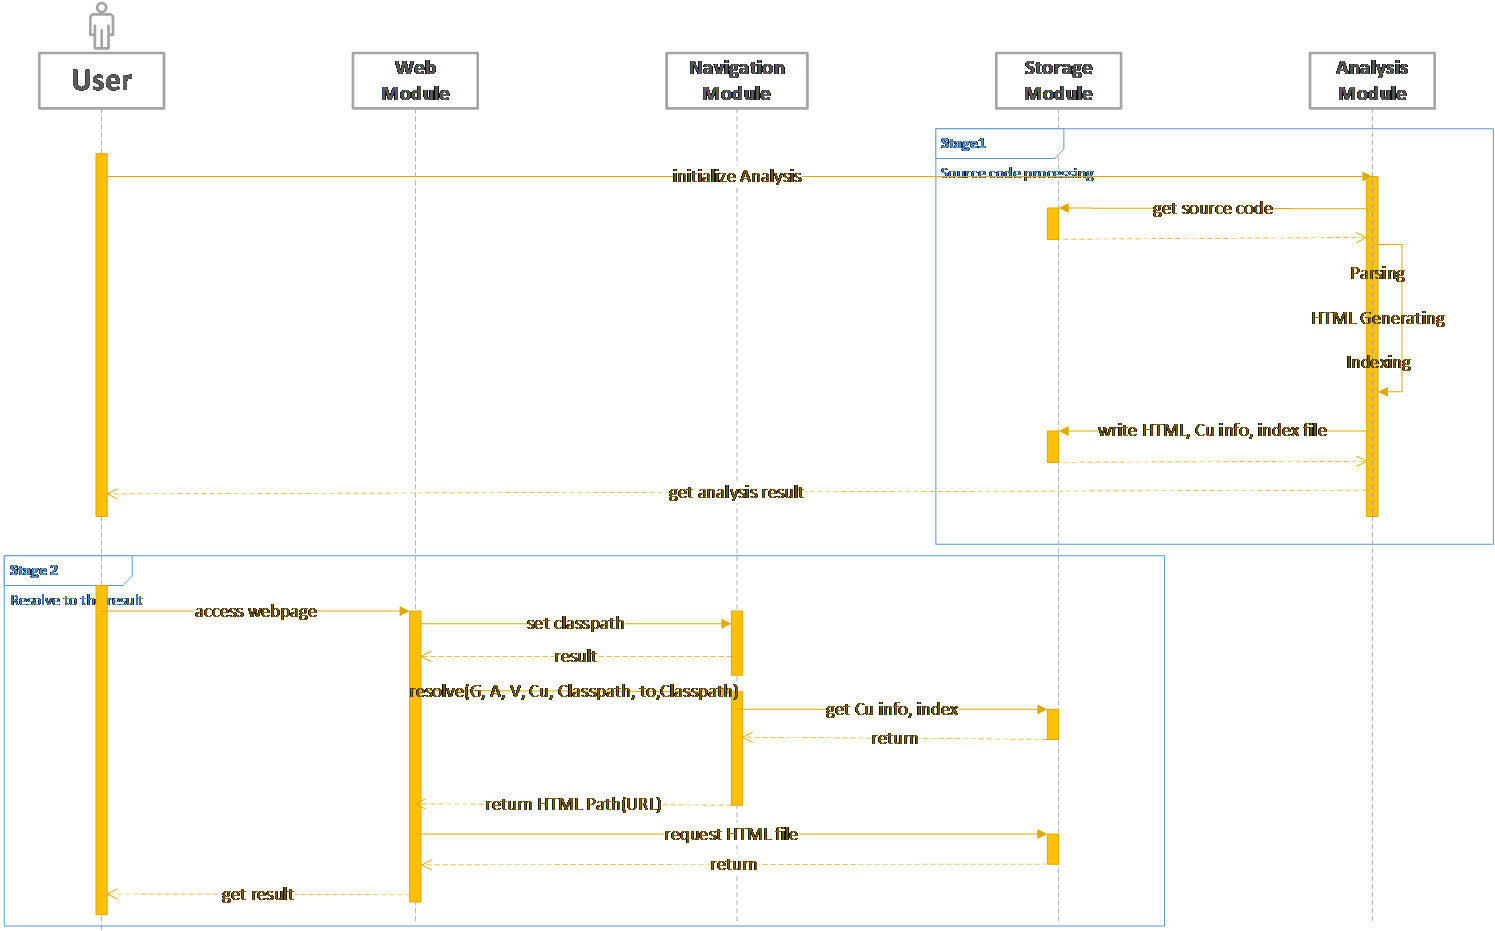
\includegraphics[width=12cm]{pic/system-uml.png}
	\caption{UML of the system}
	\label{UML of the system}
\end{figure}

With this architecture(Fig. 9), all source codes in the jar files are proceeded at the same time during the analysis stage and saved to the storage system, making it possible to provide a general resolving service in high efficiency and low expenditure.

%=============================
%===5 Source code analysis====
%=============================
\section{Source code analysis}

There are several steps within the analysis stage, which can be briefly introduced by Fig. 10.

\begin{figure}[H]
	\centering
	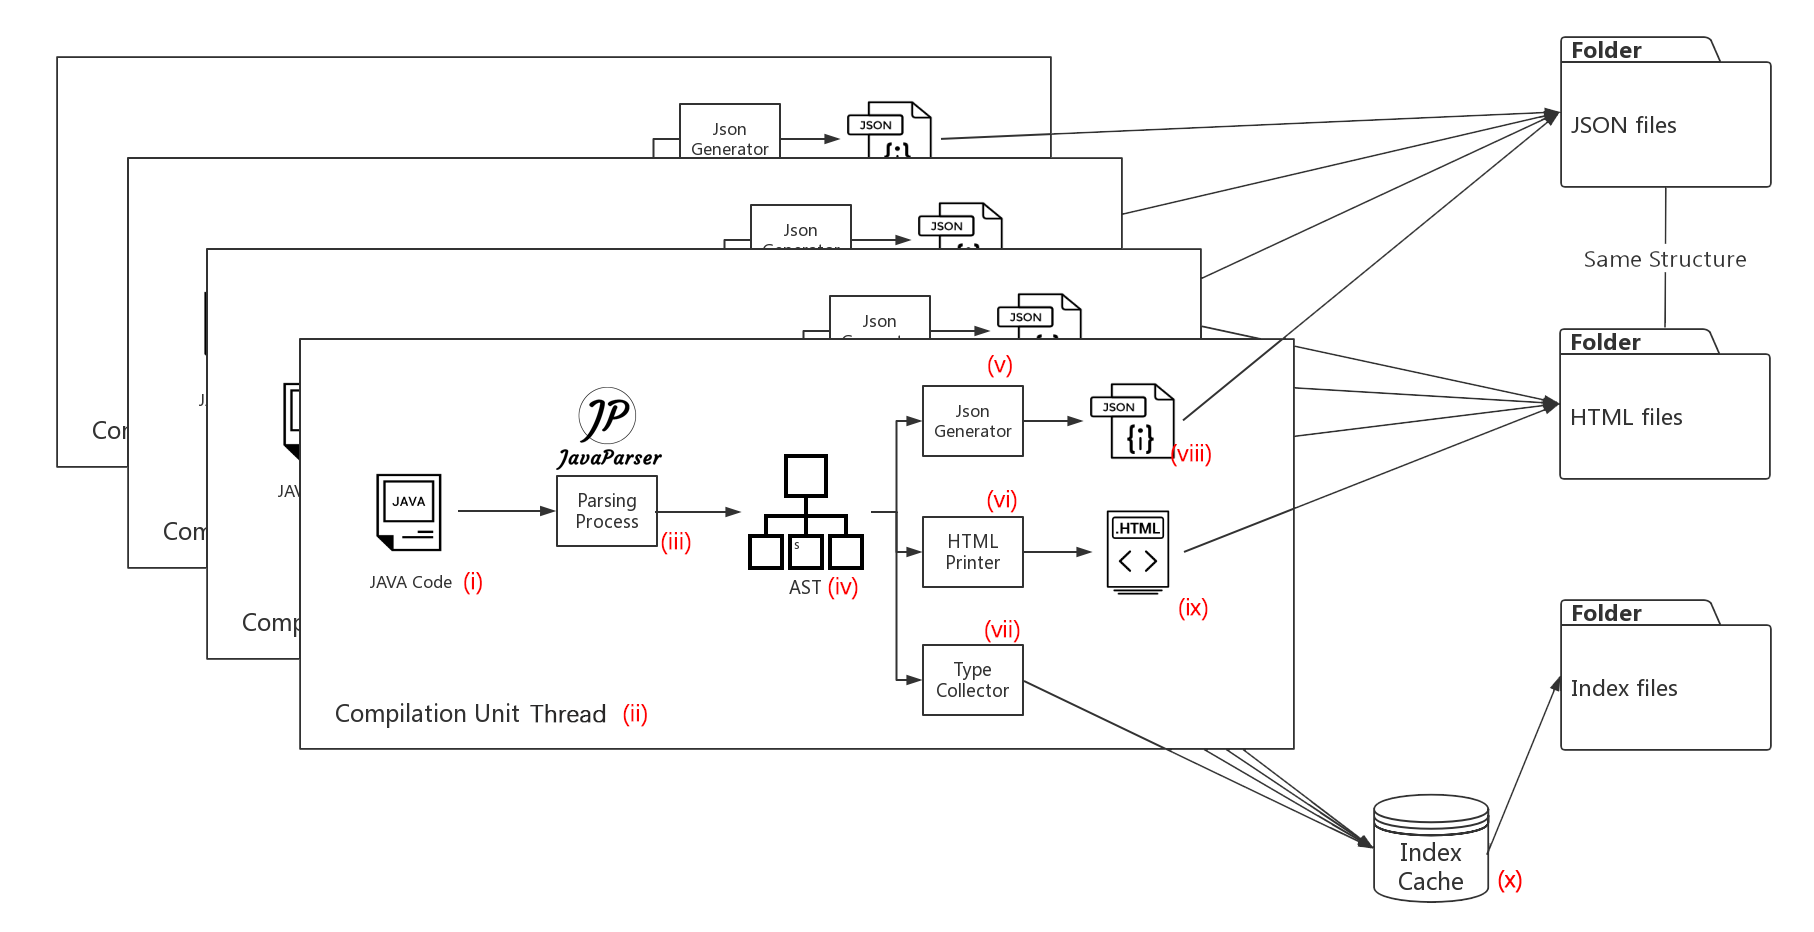
\includegraphics[width=12cm]{pic/AnalysisFlow.png}
	\caption{UML of the system}
	\label{Source code analysis process}
\end{figure}

\subsection{Source code to AST}

The source code for a Java class is organized into compilation units, and a simple compilation unit contains a single class definition and is named for that class\cite{learningJava_2013}, so firstly, the system will read every jar file within the target repository, and process every java file(i) individually in the compilation unit thread(ii). The java code will be parsed by the parsing process(iii), then generate an AST(iv) that stores all relevant information of this java file.

The AST (Abstract Syntax Tree) is a tree representation of the abstract syntactic structure of source code written in a programming language.\cite{AST_introduction} For example, “437+734” can be processed by the following steps:


\begin{figure}[H]
	\centering
	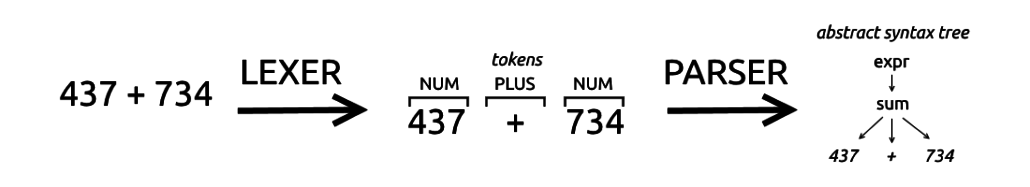
\includegraphics[width=12cm]{pic/AST-Example.png}
	\caption{Example of how lexer and parser works\cite{parsing-in-java}}
	\label{Example of how lexer and parser works}
\end{figure}

Firstly, the lexer will recognise different tokens and marks them with the meaning of these tokens, and then the parser will generate an abstract syntax tree which stores this information into every individual node. With the tree structure, we can easily trace between different nodes and find out the relation between different nodes.

This project uses Java Parser to analysis the code and generates the AST structure of the code. The JavaParser library allows you to interact with Java source code as a Java
object representation in a Java environment. More formally, it refers to this object representation as an Abstract Syntax Tree (AST).\cite{smith_javaparser:_2016}

\subsection{AST to Html}

When we got an entire AST(iv) that describe everything within specific compilation unit, the Html Printer(vi) will transform the AST(iv) into an Html file(ix), because basically the AST\cite{AST_introduction}(iv)  stores everything that comes from the raw Java file. The only difference is that the Html Printer[6] need to find out all the occurrence of every class and interface type that is used in within the code and then wrap it with “<a>” tag, so that these types will be displayed as hyperlinks for the user to click. See Appendix 1 for the relevant code. Also, Code Prettify\cite{code-prettify} is integrated with the Html file(ix)  generated by Html Printer(vi).

After this process, we can generate a single Html file(ix) that display all the java code from the raw java file(ii), like what is shown in the Fig. 12.

\begin{figure}[H]
	\centering
	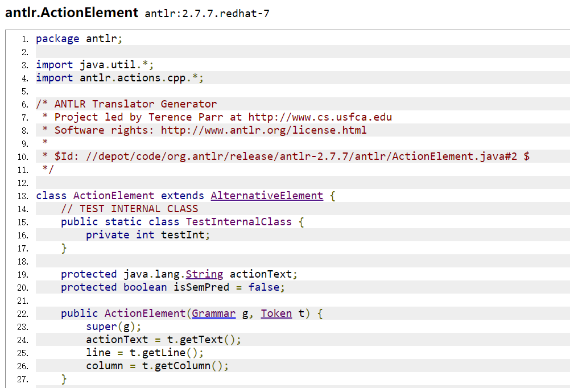
\includegraphics[width=12cm]{pic/webpage-sample.png}
	\caption{Webpage generated by AST}
	\label{Webpage generated by AST}
\end{figure}

\subsection{AST to JSON file}

A single Html file(ix) can help display the source code that stores in the java file(ii), but if the user wants to resolve the links to get the right target result, some necessary information should be generated and saved into storage system together with the Html file(ix). 

The JSON Generator(v) is a function that retrieves type declarations, import declarations and package declarations from the AST(iv), then save them as a JSON file(viii) in the storage system. For every Html file(ix), there is a JSON file(viii) with the same filename and same storage path with the Html file(ix). Here is an example of how JSON file looks like.

\subsection{AST to Index file}
If we want to resolve specific link that contains the target type name, we need to generate an index system that works as a dictionary to help the resolver know how much possible targets are there in the entire repository. So within the analysis stage of every compilation unit thread(i), the type collector(vii) will retrieve full qualified type name from the type declaration in the AST(iv) and save it to a hash map in the index cache(x).

After all jar files have been analysed, the system will iterate every item in the cache and save them into different index file named with the type name. See Appendix 1 for the relevant code.

%=============================
%===     6 Navigation     ====
%=============================
\section{Navigation}

After we analysis all Java files within the repository, the system should be available to provide a navigation service for front-end browser to redirect between different pages.

\subsection{Universal Unique Type Name(UUTN)}
It is possible that two different java files from different jar files share the same fully qualified type name. For example, “java.lang.String” may come from source code of either Java12 or Java8. In order to navigate between different java files, we need to design a file storage system that copes with the co-existence of the Java files from different versions of source code.

\begin{figure}[H]
	\centering
	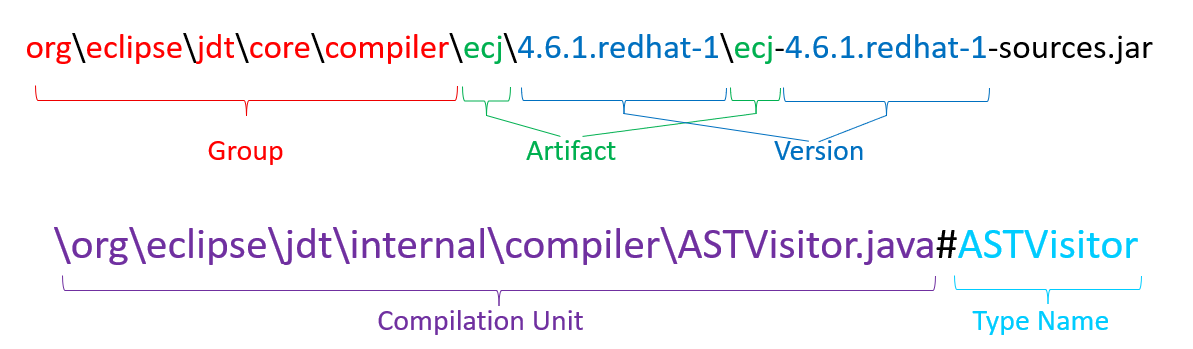
\includegraphics[width=12cm]{pic/GavCuSample.png}
	\caption{Full path of a specific Java type}
	\label{Full path of a specific Java type}
\end{figure}

The Fig. 13 shows an example of a universal unique file name of a specific Java type. It consists of five factors:

\begin{itemize}
	\item The group id of the project;
	\item artefact id of this project;
	\item The version of this product;
	\item The fully qualified name of this compilation unit;
	\item The type name of this type.
\end{itemize}

Since both Html files and JSON files are saved in this path and file name, you can locate any Java type with the entire repository with these five factors.

\subsection{Resolve Function}
When user trying to navigate from specific Java file to another Java file that via the hyperlink, it should pass the UUTN of current Java file (which is regarded as “navigate from”) and the target type name(which is regarded as “navigate to”) to the backend server. A typical resolve request may look like this:

\begin{lstlisting}[language=Java, caption=Resolver example]
Resolver.resolve(groupId, artifactId, version, compilationUnit, typeName, navTo){/*...*/}
\end{lstlisting}

The groupId, artifactId, version, compilationUnit and typeName parameter are exactly the UUTN of where you navigate from, and the navTo represent the String of the type name of your target.

\subsection{Priorities for Resolving}

As what was mentioned in paragraph 2.2, there is no existing research defines a general rule of how to resolve the type name and navigate to the right target Java type that is quoted by current scope. Thus a cross-validation test was conducted to all different kinds of references.

This test is designed some cases with different type with same type name but imported differently. For example, in Listing 1.2, we explicitly imported class Type from package org.myproj, and at the same time declared a nested type named Test as well, then we compile and run the code to figure out which class is actually used by current type. 

\begin{lstlisting}[language=Java, caption=Sample code to show the complexity of Java]
	package Test1;

	//This is a specific imported class Test;
	import org.myproj.Test;
	
	public class ImportTest {
		Test test = new Test();
		class Test {
			// This is a Nested Class Test;
		}
	}
\end{lstlisting}

The result of the cross-validation is shown as below:

\begin{figure}[H]
	\centering
	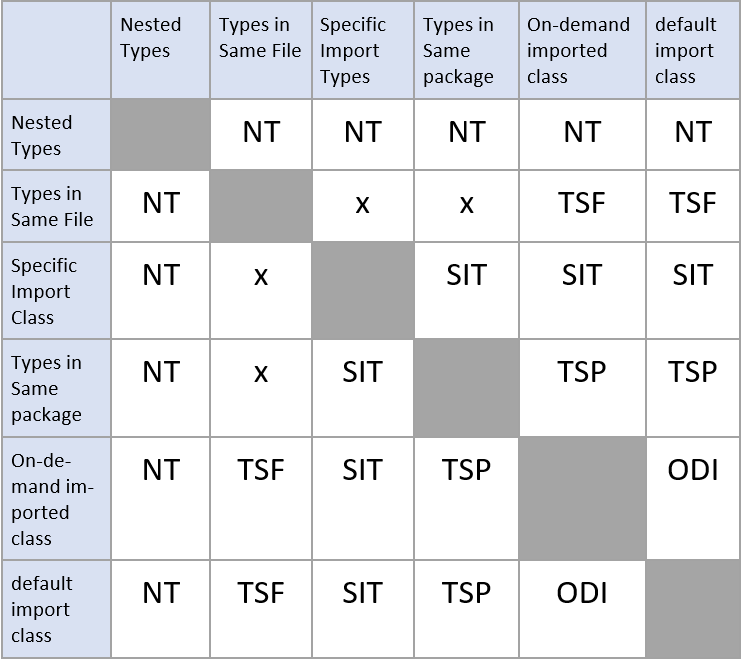
\includegraphics[width=12cm]{pic/cross-validation-result.png}
	\caption*{*NT: Nested Types, TSF: Types defined in the Same File, SIT: Specific Imported Types, TSP: Types in the Same Package, ODI: On-demand Imported types}
	\caption*{**Result marked with x means this kind of combination is impossible to occur.}
	\caption{Cross-validation result}
	\label{Cross-validation result}
\end{figure}

According to the result of the cross-validation, there are seven steps to resolve any target of Java types:

\begin{enumerate}
	\item Find if it has the same name with current Type (Class / Interface) itself;
	\item Find all nested Types and Types that defined in same java file;
	\item Find specific-imported type;

	e.g., import uk.ac.ncl.cs.tongzhou.navigator.learnning.testpackage.Date;
	\item Find Types defined in the same package;
	\item Find on-demand imported types;

	e.g., import uk.ac.ncl.cs.tongzhou.navigator.learnning.testpackage.*;
	\item Find in all default imported packages 
	, e.g., String from java.lang
	\item Find directly nominated type, e.g.,  java.util.Date date=null.
\end{enumerate}

These seven rules can help the resolver to find out the right target without Java compiler or JVM, which gives an unobstructed waterflow to resolve some specific type name into the correct target that been referred by current Type.

\subsection{User-customised classpath}
In paragraph 6.1, we introduced UUTN(Universal Unique Type Name), which is a method that uses group id, artefact id, version, compilation unit name and type name to find any type within the system. But if you want to locate a specific jar file, you only need G(Group), A(artefact), V(version) to specify a particular version of some open-source project.

Classpath information is just a set of GAVs that defines which jar files are included in the customized scope the user wants to use during the resolving process. Since the classpath list might be pretty long, users need to save their own classpath to the server so that they can use it every time they access the system.


\begin{figure}[H]
	\centering
	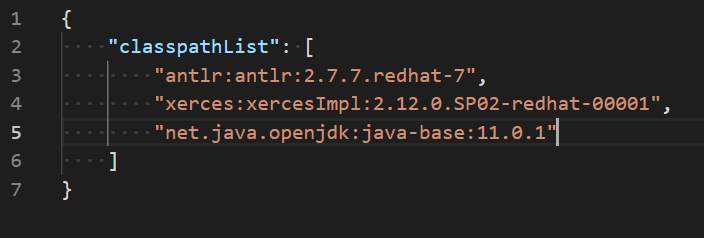
\includegraphics[width=10cm]{pic/classpath-json.png}
	\caption{Sample of a classpath Json file}
	\label{Sample of a classpath Json file}
\end{figure}

However, as was shown in Fig. 15, different users share a single server (or server group), if the server uses a general classpath file, the operation from different users may have interference with each other.

To solve this problem, when the user uploads their customised classpath, the system will actually generate the hash code from the classpath, name the classpath file with this hash code and save the file into the storage system, then finally send the response back to the browser with this hash code. The front-end script will create a new item in the cookie named “classpath-hash” and save the hash code to the value.

\begin{figure}[H]
	\centering
	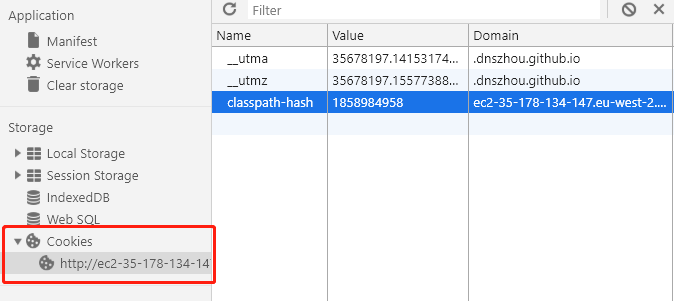
\includegraphics[width=10cm]{pic/cookie-storage.png}
	\caption{Hash code saved in cookie storage}
	\label{Hash code saved in cookie storage}
\end{figure}

Then every time the front-end trying to resolve any link, it will bring the cookie information to the server. The server can find the right classpath file according to the cookie information with the request, then resolve the link correctly according to the classpath information.

%=============================
%===   7 Cloud Solution   ====
%=============================
\section{Cloud Solution}

To provide service to users from all over the world, a good cloud structure is pretty crucial during both deployment stage and development stage. There are different kind of solutions to choose from. All these solutions have their advantages and disadvantages. Thus an evaluation of these solutions was conducted during this project.

\subsection{EC2 + EBS}


Amazon Elastic Compute Cloud (Amazon EC2) provides scalable computing capacity in the Amazon Web Services (AWS) cloud.\cite{AWSEC2}

Amazon Elastic Block Store (EBS) is an easy to use, high-performance block storage service designed for use with Amazon Elastic Compute Cloud (EC2) for both throughput and transaction-intensive workloads at any scale.\cite{AWSEBS}

\begin{figure}[H]
	\centering
	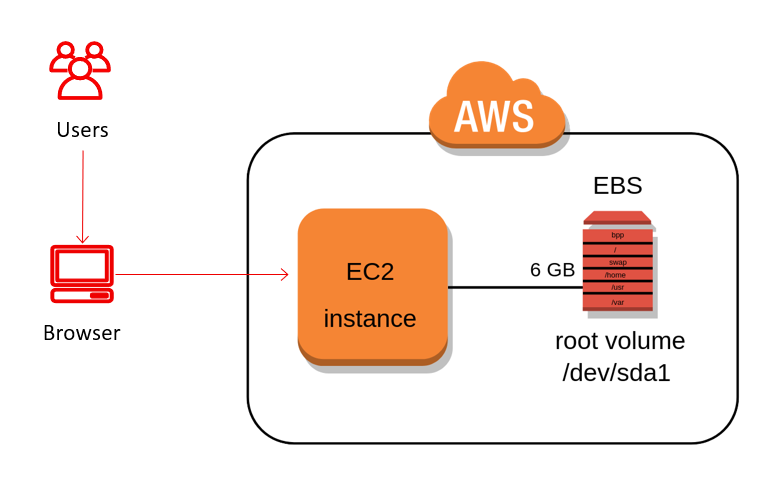
\includegraphics[width=10cm]{pic/ec2-ebs.png}
	\caption{EC2 + EBS solution}
	\label{EC2 + EBS solution}
\end{figure}

This is the easiest cloud solution to implement because using EC2 and EBS is just like using a virtual machine with a high-speed hard disk volume automatically mounted to the system.

To examine the solution we chose a free-tier server type with one core CPU and 1GiB memory, according to the requirement defined in paragraph 2.3-5b.

\begin{figure}[H]
	\centering
	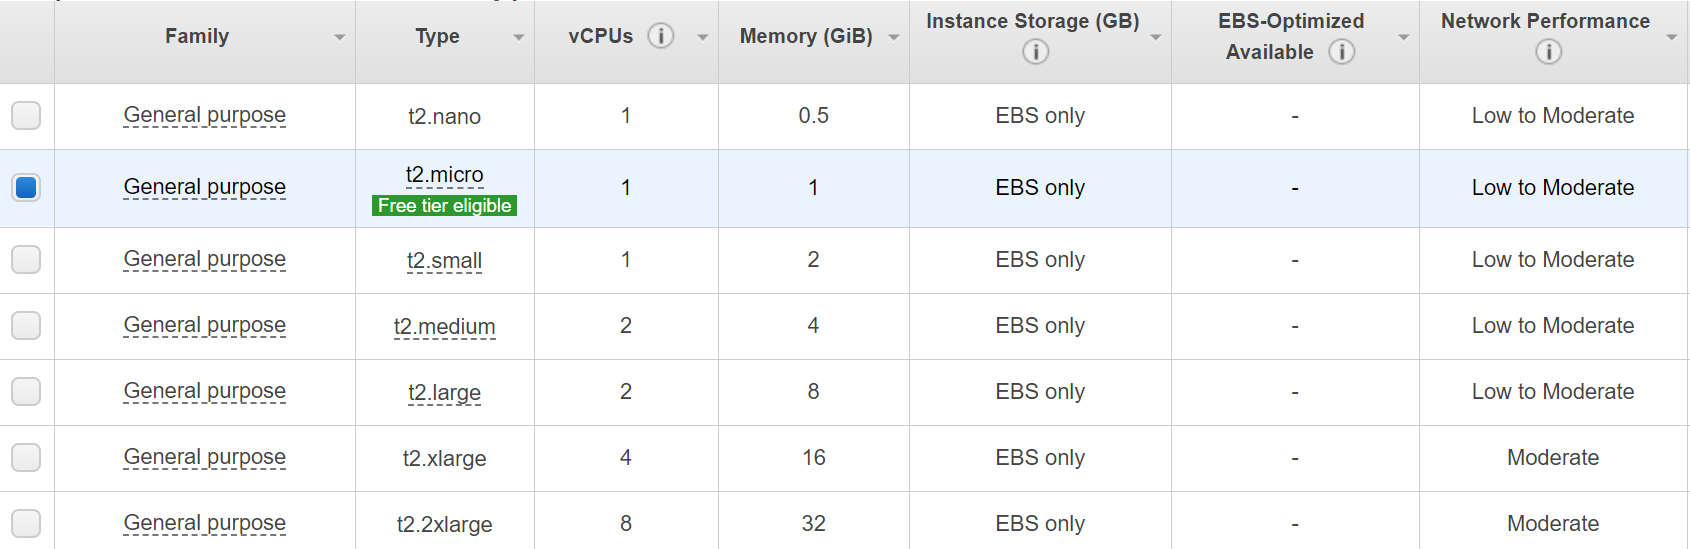
\includegraphics[width=10cm]{pic/ec2-free-tier.png}
	\caption{Diiferent configurations of AWS EC2 instances}
	\label{Diiferent configurations of AWS EC2 instances}
\end{figure}

This solution provided a nice performance(see paragraph 8.3-1), which is the best one among all the solutions under the performance test because EBS is a high-performance block storage service that works better than traditional hard disk.

But with this solution the cost of storage may become really high, because Amazon EBS pricing is based on its use for high-performance workloads, it can be expensive for data that doesn’t require access via highly performant disks.\cite{ebs-efs-amazons3} It is also tricky for system administrator to increase the storage if there are new source code to be analysed in the repository.

Another disadvantage of this solution is that we can not integrate EBS volume with CDN(Content Delivery Network)\cite{Content_delivery_network} system, which may cause a latency when global users are trying to access our system.

\subsection{EC2 + S3}

Amazon Simple Storage Service (Amazon S3) is an object storage service that offers industry-leading scalability, data availability, security, and performance.\cite{amazons3}

\begin{figure}[H]
	\centering
	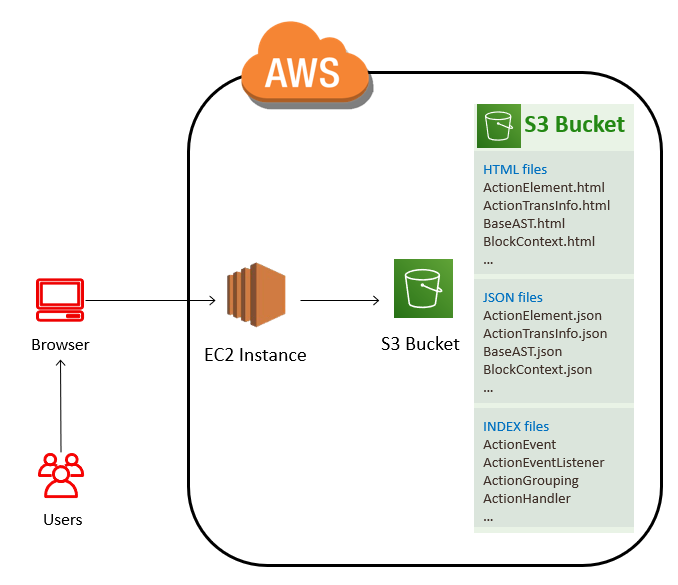
\includegraphics[width=10cm]{pic/ec2-s3.png}
	\caption{EC2 + S3 solution}
	\label{EC2 + S3 solution}
\end{figure}

With this solution, all data were stored in S3 bucket, and the program within EC2 instances access S3 directly to retrieve relevant data. 

Since S3 can be easily integrated with CDN service, this solution can ensure the accessibility are equally from all over the world. 

But actually, the cost of this solution may increase exponential, because of the pricing rules of S3 product. (see Appendix 3) It not only charges for storage but also charges for requests that exchanged with S3 bucket, no matter the request comes from EC2(internal AWS network) or from user browser.

Another problem of S3 solution is about the performance, the access from EC2 to S3 is actually worse than the access to EBS(see paragraph 8.3), because EBS is directly attached to EC2, and for S3 there are a lot of validation rules which cost more time than EBS.

\subsection{Lambda + API Gateway + S3}
Another popular solution is the serverless architecture that using API Gateway\cite{api-gateway} to accept Http requests and redirect to AWS Lambda\cite{lambda} service to process and interact with the S3 storage system.

\begin{figure}[H]
	\centering
	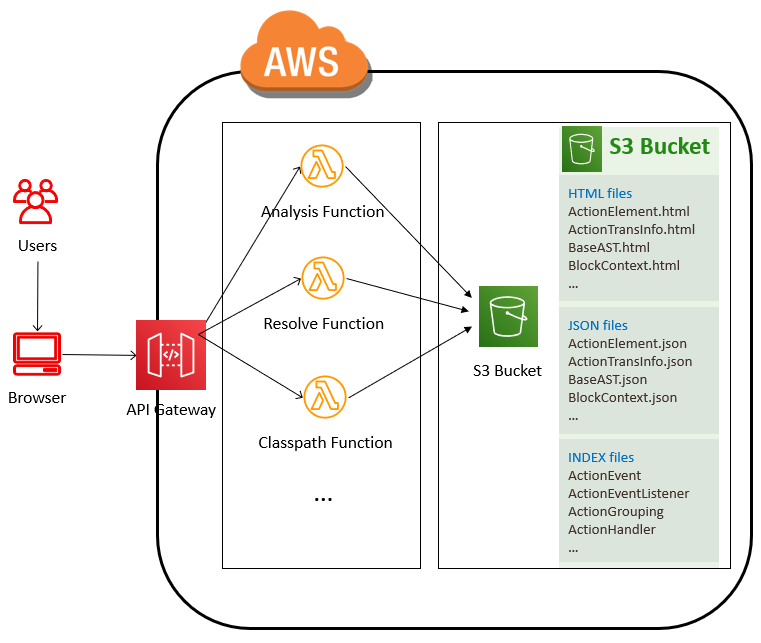
\includegraphics[width=10cm]{pic/lambda-s3.png}
	\caption{Lambda + API Gateway + S3 solution}
	\label{Lambda + API Gateway + S3 solution}
\end{figure}

AWS Lambda lets you run code without provisioning or managing servers. You pay only for the compute time you consume - there is no charge when your code is not running.

Although Lambda supports a lot of different programming language, it does not work perfectly with Java code. You can not debug Java code online like Node.js or other supported languages, and the platform support only Java version 8, while our project was developed with Java12.

Also, it is challenging to apply CI(Continuous Integration)\cite{Continuous_integration} tools to Lambda services because all the codes are separately in different Lambda functions.

\subsection{EC2 + EBS + S3}

After investigation EC2, EBS, S3, Lambda and other relevant cloud solutions, we decided to build a hybrid architecture that takes advantages from both S3 solution and EBS solution, which is shown in following diagram.

\begin{figure}[H]
	\centering
	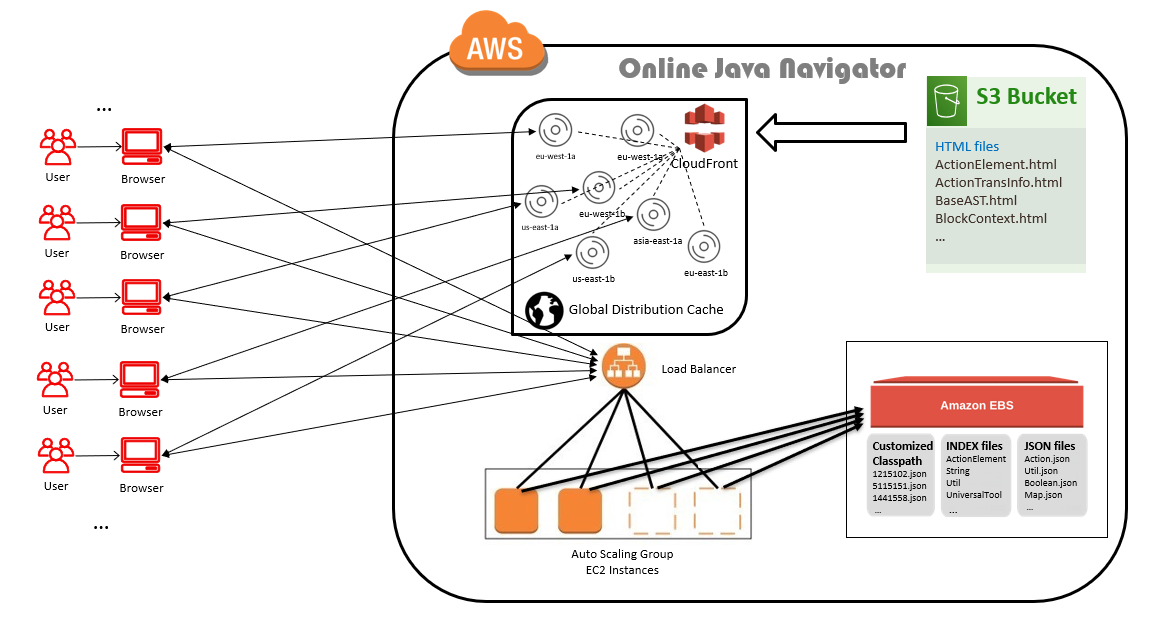
\includegraphics[width=12cm]{pic/ojn-cloud-solution.png}
	\caption{Topology of Online Java Navigator}
	\label{Topology of Online Java Navigator}
\end{figure}

As is presented in Fig. 21, there are different steps to finish the entire process:

\begin{enumerate}
	\item Different users can use their own browser to access our website;
	\item When user click the link, the browser send a request to the load balancer;
	\item The load balancer will find a server with the lowest capacity to process the request
	\item The server within the EC2 instance retrieves the right classpath file from EBS
	\item The server looks up the index file and JSON file in EBS to resolve the link
	\item The server returns the right path of the type back to the front-end browser
	\item The Browser retrieves the target Html file from the global distribution cache that generated from the S3 bucket.

\end{enumerate}

If all EC2 instances are under high capacity, the auto-scaling group will initialise another EC2 instance and connect it to the load balancer, which makes sure that every user can access the system with highest accessibility.

To enable this kind of auto-scaling structure, the system is required to be designed as a stateless program. Every time a user resolve any type in our system, the request send to backend actually have everything needed for resolver to get the result, which means every request is independent with each other.

Also, with this structure, the number of access request from EC2 to S3 are minimised. With the EC2 + S3 solution introduced in paragraph 7.2, for every request there will have at most three get request directed to S3 bucket, which is retrieving the JSON file, the index file and the Html file. With Hybrid solution, the only request to S3 bucket is the get request for Html file from user browser, which means the amount of the request has been reduced by two-thirds. As we discussed in paragraph 7.2, the access to S3 is actually slower than the access to EBS, so this hybrid solution obviously improves the performance of this system(see paragraph 8.3 for the testing result).

On the other hand, since AWS charge the S3 service by the amount of the request that sends to S3, this hybrid solution saves many budgets and at the same time achieves even better performance.

%=============================
%===   8 Evaluation   ====
%=============================
\section{Evaluation}

\subsection{Unit Testing \& Integrate Testing}

Unit testing is a software testing method by which individual units of source code, sets of one or more computer program modules together with associated control data, usage procedures, and operating procedures, are tested to determine whether they are fit for use.\cite{huizinga2007automated} Junit tool was integrated into this project to perform unit testing and integrate testing during the development stage.

Different type of test cases was designed to cover as much code as possible. In Fig. 22 it shows the coverage of the code that was involved by Junit test cases, and most of those core classes that marked in blue were covered in a high coverage.

\begin{figure}[H]
	\centering
	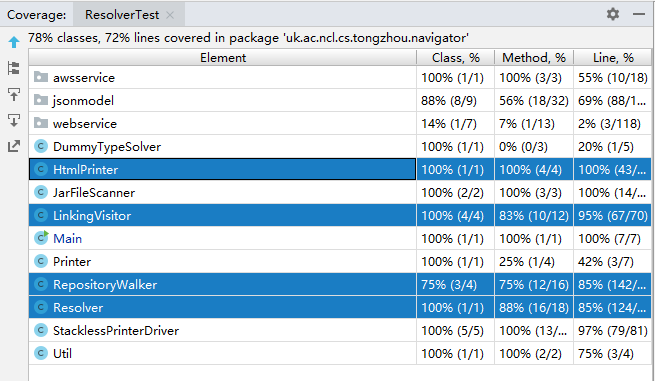
\includegraphics[width=12cm]{pic/unit-test-coverage.png}
	\caption{Coverage analysis of the test cases}
	\label{Coverage analysis of the test cases}
\end{figure}

During the development stage of the project, these test cases also worked as a kind of regression test. Regression testing is re-running functional and non-functional tests to ensure that previously developed, and tested software still performs after a change.\cite{basu2015software} Since different functions are developed separately, and different functions may have internal relationship with each other, it is especially important to make sure that newly developed functions do not ruin any existing function in the system.

\subsection{Automation Testing}
Since this navigator generates links for every Type that occurred in the java code, it is important to know how much links can be resolved appropriately, which can reflect the accuracy of the resolving system.

Thus an automation testing program was developed for this product. As what is shown in the Fig. 10 in paragraph 5, the AST was generated by parsing process and contained all relevant information of the source code, so the server also produced a list of test cases that describe every available link as G,A,V,Cu,TypeName and NavigateTo, and save them into CSV files.

In the Junit test folder, there is a testing program that loads all the test cases and passes it to resolving function, so that it can cover every link in the system and test them automatically.


\begin{figure}[H]
	\centering
	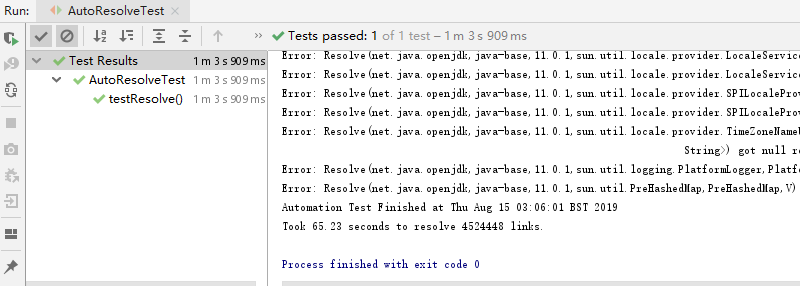
\includegraphics[width=12cm]{pic/automation-test.png}
	\caption{The result of the automation test}
	\label{The result of the automation test}
\end{figure}

\subsection{Performance Testing}
Performance testing is, in general, a testing practise performed to determine how a system performs in terms of responsiveness and stability under a particular workload.\cite{performance_testing} Since this project is designed to provide service to different users at same time, so it is especially important to examine how the system works when multiple user access the system.

To carry out this test, JMeter\cite{halili2008jemeter} tool is used during the performance testing stage. Apache JMeter is an Apache project that can be used as a load testing tool for analysing and measuring the performance of a variety of services, with a focus on web applications.\cite{Apache_JMeter} We set the testing parameter as follow:

\begin{itemize}
	\item Threads: 20;
	\item Ramp-Up Time: 5 seconds;
	\item Loops: 20
\end{itemize}

Which means the JMeter will initial 20 user threads within 5 seconds, and it will test every API for 20 times. During the testing stage, three different solutions were tested as a comparison.

\subsubsection{EC2 + EBS solution}

\begin{figure}[H]
    \centering
    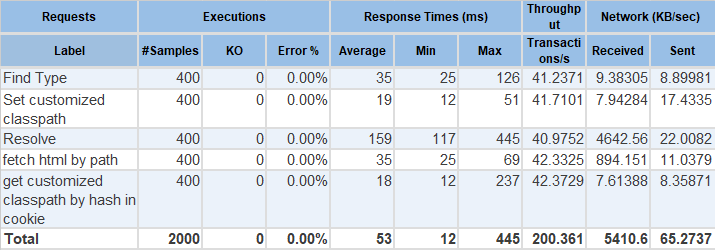
\includegraphics[width=11cm]{pic/jmeter-ebs.png}
    \caption{Result of 20 thread performance testing with EC2 + EBS solution}
    \label{Result of 20 thread performance testing with EC2 + EBS solution}
\end{figure}

This solution got the best result in terms of the performance, the average response time is only 53ms, and the total throughput is 200.361 transactions per second.

\subsubsection{EC2 + S3 solution}
\begin{figure}[H]
    \centering
    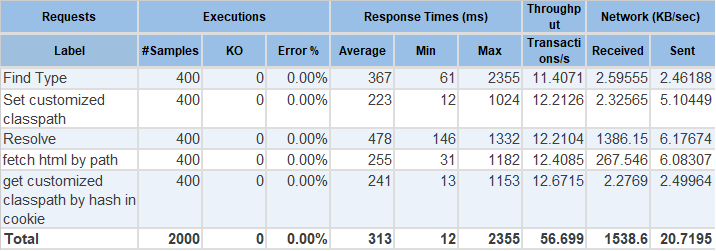
\includegraphics[width=11cm]{pic/jmeter-s3.png}
    \caption{Result of 20 thread performance testing with EC2 + S3 solution}
    \label{Result of 20 thread performance testing with EC2 + S3 solution}
\end{figure}

When the entire storage system was moved to S3, the performance became much worse than that on EBS. On average, it took 313ms to process every request, and the average throughput decreased to 56.699 transactions per second, only a quarter as much as that with EBS solution.

\subsubsection{EC2 + EBS + S3 hybrid solution}
\begin{figure}[H]
    \centering
    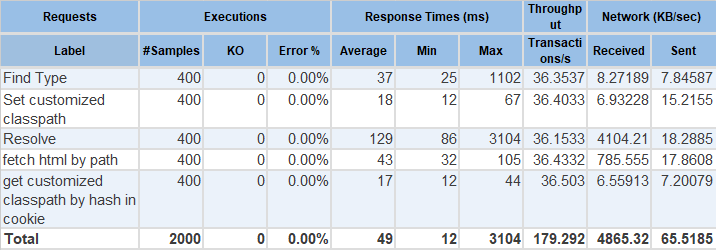
\includegraphics[width=11cm]{pic/jmeter-hybrid.png}
    \caption{Result of 20 thread performance testing with Hybrid solution}
    \label{Result of 20 thread performance testing with Hybrid solution}
\end{figure}

With a hybrid solution, the average response time was 49 ms, similar to the EBS solution. The throughput was 179.292 transactions per second, a little bit less than EBS solution, but much better than the S3 solution.

\subsubsection{High capacity testing}
To examine the performance of the product under a higher capacity, another test plan was executed to both EBS solution and EBS + S3 hybrid solution.

\begin{itemize}
	\item Threads: 100;
	\item Ramp-Up Time: 10 seconds;
	\item Loops: 20
\end{itemize}

\textbf{EBS solution:}
\begin{figure}[H]
    \centering
    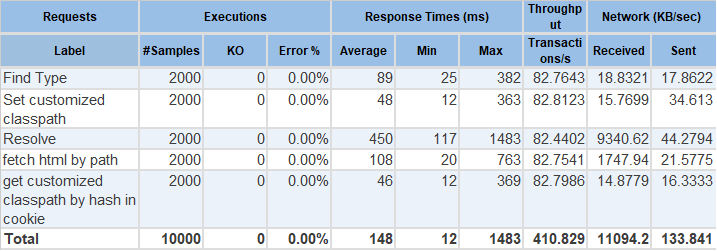
\includegraphics[width=11cm]{pic/jmeter-100-ebs.png}
    \caption{Result of 100 thread performance testing with EC2 + EBS solution}
    \label{Result of 100 thread performance testing with EC2 + EBS solution}
\end{figure}

\textbf{Hybrid solution:}
\begin{figure}[H]
    \centering
    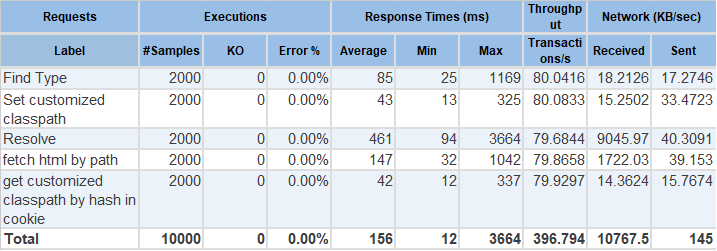
\includegraphics[width=11cm]{pic/jmeter-100-hybrid.png}
    \caption{Result of 100 thread performance testing with Hybrid solution}
    \label{Result of 100 thread performance testing with Hybrid solution}
\end{figure}

With higher capacity, both these two solutions work similarly. The Hybrid solution seems to be a little bit worse than EBS solution in terms of average response time and throughput.

\subsection{Project Management}
Although this project was conducted by one person only, it is still important to adopt an appropriate methodology that helps to manage the entire development process.

Traditional develop team take waterfall\cite{Waterfall_model} model to manage the development life-cycle so that they can clearly research, design, develop, test and deploy the product in separate stages. This model makes the develop progress tracked explicitly, but with the development of software engineering, it takes less time to develop software products. On the other hand, the requirement of the software product is frequently changing, which is almost a disaster to traditional waterfall model.

While Scrum\cite{Scrum} model is such a kind of methodology that was designed to follow up the changing market. In this project, we use a professional tool, Jira\cite{jira}, to help track and manage the entire development plan.

\begin{figure}[H]
    \centering
    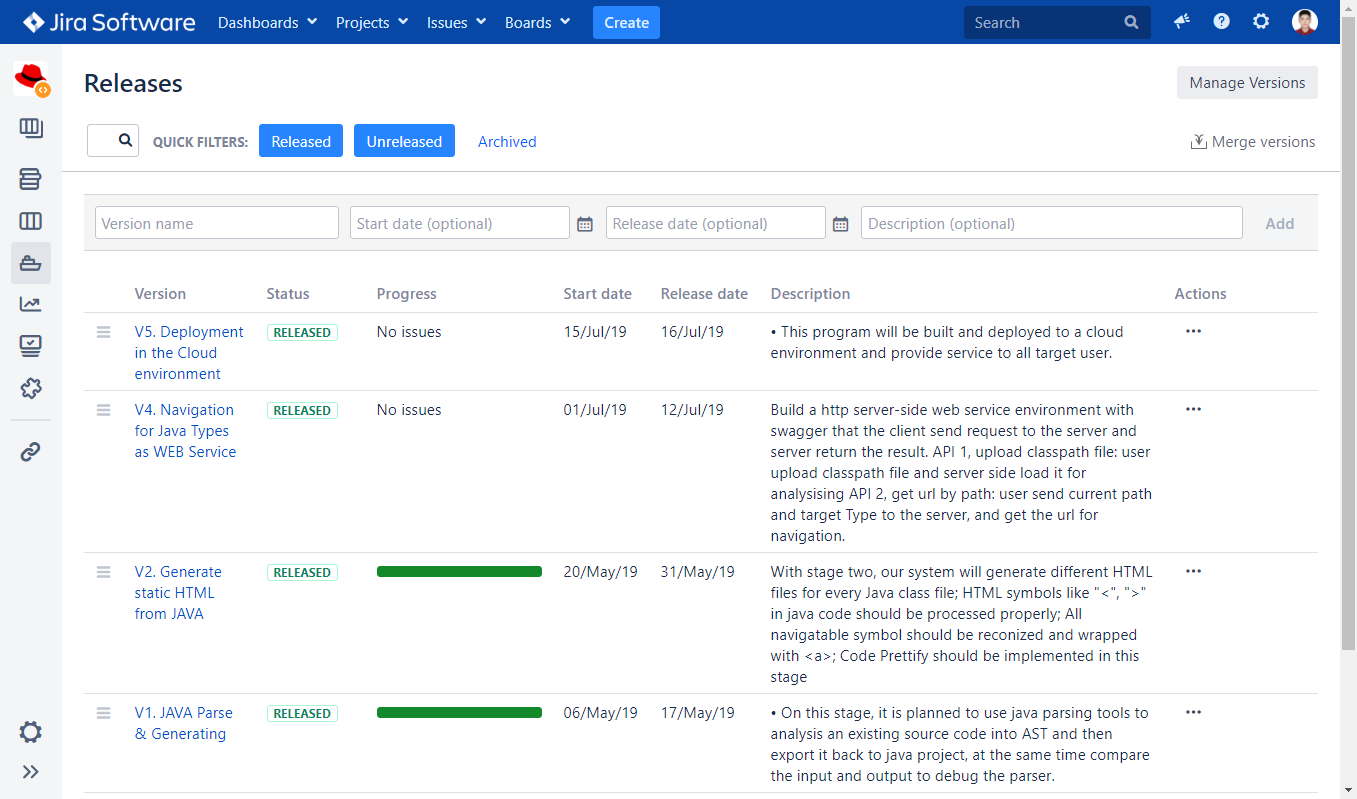
\includegraphics[width=11cm]{pic/jira.png}
    \caption{Jira tool release management page for this project}
    \label{Jira tool release management page for this project}
\end{figure}
In this project, there was four separate sprint which achieved different goals and published several successful releases. 

\begin{figure}[H]
    \centering
    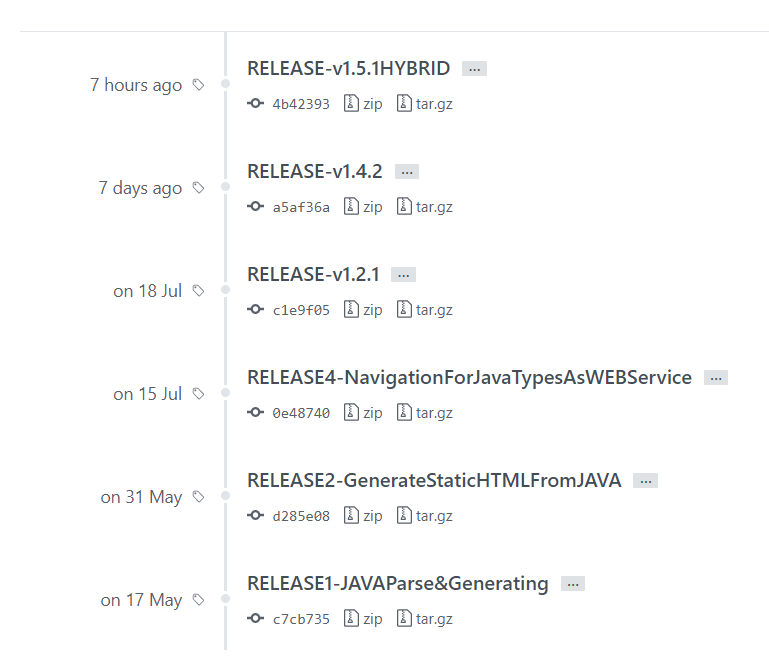
\includegraphics[width=8cm]{pic/github-release.png}
    \caption{All releases delivered for this project\cite{ojn-releases}}
    \label{All releases delivered for this project}
\end{figure}

The most crucial benefit of apply Scrum methodology comes from the flexibility of Scrum. During the project, every two weeks were regarded as an individual sprint, and after each sprint you can think over the entire project and modify the goal and tasks of next sprint. 

For example, before the start of the project, we designed another sprint which aimed to deliver some edge feature like function navigation, but after sprint 2 we found that the type navigation function spent more effort than expected. In order to deliver the entire product on time, the scope and the sprint target was modified, and some edge features were discarded. If we adopted waterfall model, there would have no room to alter the scope after we started the project.
	
%=============================
%===   9 Conclusion   ====
%=============================
\section{Conclusion}
This project finished with the Online Java Navigator been developed and deployed to AWS successfully, and 97.12\% of the links can be resolved, according to the automation test. There are a lot of significance and contributions achieved from this project, and also there are rooms for future improvements.

\subsection{Significance and Contribution}
This project delivered precisely what Red Hat customer want, an exclusive web-based source code navigator with a configurable classpath for the user to use.  Currently, it is the only open-source product that providing service to all developers.

The optimized cloud solution with both EBS and S3 make it possible to provide service to as many users as possible and at the same time, reduce as much cost of cloud services as possible.

The two-stage structure of the system makes it easy to integrate the system with any other code repository. You can easily change the result of the resolving from S3 bucket to any repository link like GitHub, and then it can leverage any existing Java code browsing system with the ability to navigate from different types.

\subsection{Limitation and defects}
The time limit was the most significant problem because it takes much time to understand the requirement, research on different technology, develop the software product and debug it. Thus a lot of useful features, such as method navigation and integration with the third-party website, was discarded due to the limitation of the time.

Another limitation was the lack of knowledge and experience on Computational linguistics and the mechanism of Java compiling. It took much time to understand those basic concepts and theory and apply them into practice.

Also, due to some defect from the open-source product we use like Java Parser, there may have some defects that difficult to fix. 

\subsection{Future improvements}
There are still some defects within the system, so firstly we will try to fix them in the following versions.

Also, a lot of useful functions will be developed, such as directly upload local ".classpath" file from Eclipse and load it to our system.

Last but not least, the parsing and resolving algorithms will be improved to provide better performance to the user.


\newpage
\bibliographystyle{plain}
\bibliography{reference}

\newpage
\section*{Appendix 1: Relavant source code }
\addcontentsline{toc}{section}{Appendix 1: Relavant source code}

\begin{lstlisting}[language=Java, caption=Retrieve all occurrence of class and interface type during visiting]
//uk.ac.ncl.cs.tongzhou.navigator.LinkinVisitor.java

	@Override
    public void visit(ClassOrInterfaceType node, JavaSymbolSolver javaSymbolSolver) {

        SimpleName simpleName = node.getName();
        String fullName = node.getTokenRange().get().toString();
        if (fullName.contains("<")) {
            fullName = fullName.replaceAll("<.*>", "");
        }
        String navFrom = findRelativePath(node);
        LinkObject linkObject = new LinkObject(navFrom, fullName);
        simpleName.setData(LINK_TO, linkObject);
        simpleName.setData(LINK_STYLE, "ClassOrInterfaceType");

    }

\end{lstlisting}

\begin{lstlisting}[language=Java, caption=Retrieve type declaration during visiting]
//uk.ac.ncl.cs.tongzhou.navigator.LinkinVisitor.java
	
public class LinkingVisitor extends VoidVisitorAdapter<JavaSymbolSolver> {

    public static final DataKey<String> LINK_STYLE = new DataKey<>() {
    };
    public static final DataKey<String> LINK_ID = new DataKey<>() {
    }; // for origins
    public static final DataKey<LinkObject> LINK_TO = new DataKey<>() {
    }; // for targets

    private final List<TypeDeclaration> typeDeclarations = new ArrayList<>();
    private final List<ImportDeclaration> importDeclarations = new ArrayList<>();

    private final List<String> declaredTypes = new ArrayList<>();
    private final List<String> declaredImports = new ArrayList<>();

    public List<ImportDeclaration> getImportDeclarations() {
        return importDeclarations;
    }
    public List<String> getDeclaredTypes() {
        return declaredTypes;
    }


    @Override
    public void visit(ClassOrInterfaceDeclaration node, JavaSymbolSolver javaSymbolSolver) {

        typeDeclarations.add(node);

        ResolvedReferenceTypeDeclaration resolvedReferenceTypeDeclaration = javaSymbolSolver
                .resolveDeclaration(node, ResolvedReferenceTypeDeclaration.class);
        String name = resolvedReferenceTypeDeclaration.getQualifiedName();

        node.setData(LINK_ID, name);
        node.setData(LINK_STYLE, "ClassOrInterfaceDeclaration");

        this.declaredTypes.add(name);

        super.visit(node, javaSymbolSolver);
	}
	
	/*...*/
}
\end{lstlisting}

\begin{lstlisting}[language=Java, caption=Generate index file]
//uk.ac.ncl.cs.tongzhou.navigator.RepositoryWalker.java

private void indexRepository() throws IOException {
	//scan all the package.json file in the output/JsonDocs folder and generate index into index/ folder
	/*
	Index format:
	<group>:<artifact>:<version>:<declaration name>
	eg  antlr:antlr:2.7.7.redhat-7:antlr.actions.cpp.ActionLexer
	 */
	Files.createDirectories(outputIndexRootDir.toPath());
	Files.walkFileTree(outputJsonRootDir.toPath(), new SimpleFileVisitor<Path>() {

		@Override
		public FileVisitResult visitFile(Path file, BasicFileAttributes attributes) throws IOException {

			//Todo: think about whether change it to a special name
			if (file.toFile().isFile() && file.toFile().getName().equals("package.json")) {
				String relativePath = file.toString()
						.replace(outputJsonRootDir.getPath(), "")
						.replace(SLASH + "package.json", "");

				//To solve the separator problem with regular expression
				String[] pathTokens = relativePath.substring(1).split(SLASH.equals("\\") ? "\\\\" : SLASH);

				String artifact = pathTokens[pathTokens.length - 3];
				String version = pathTokens[pathTokens.length - 2];
				String group = relativePath.substring(1)
						.replace(SLASH + artifact + SLASH + version + SLASH + artifact + "-" + version, "");
				group = group.replace(SLASH, ".");
				PackageInfo currentPackageInfo = objectMapper.readValue(file.toFile(), PackageInfo.class);
				for (CompilationUnitDecl cuItem : currentPackageInfo.compilationUnitDecls) {
					for (TypeDecl typeDecl : cuItem.typeDecls) {
						String typeName = typeDecl.name.substring(typeDecl.name.lastIndexOf(".") + 1, typeDecl.name.length());
						String gavCuString = group + ":" + artifact + ":" + version + ":" + typeDecl.name;
						IndexType.addIndexItem(typeName, gavCuString);
					}
				}
			}
			return FileVisitResult.CONTINUE;
		}
	});
	IndexType.generateIndex();
}
\end{lstlisting}

\begin{lstlisting}[language=Java, caption=Main navigation algorithm]
//uk.ac.ncl.cs.tongzhou.navigator.Resolver.java

public String resolve(String groupId, String artifactId, String version,
                          String compilationUnit, String navigateFrom, String navigateTo, List<String> classpathGAVs) throws IOException {
        this.currentClasspathGavs = classpathGAVs;
        GavCu navigateFromGavCu = new GavCu(groupId, artifactId, version, compilationUnit);

        /*Get information of current Type from GavCu*/
        CompilationUnitDecl cuDecl = getCompilationUnitDecl(navigateFromGavCu);
        String navFromPkg = getPackage(cuDecl);
        List<ImportDecl> navFromImports = getImports(cuDecl);
        List<TypeDecl> navFromTypeDecls = getTypeDecls(cuDecl);
        String fullNavFromString = compilationUnit.substring(0, compilationUnit.lastIndexOf(".") + 1) + navigateFrom;

        /*====Rule 1: Current Type itself*/
        if (navigateTo.equals(subStringLastDot(navigateFromGavCu.cuName.replace(navFromPkg + ".", "")))) {
            return validateAndMakePath(Arrays.asList(navigateFromGavCu).stream(), null);
        }

        /*====Rule2: target type is an nested type of current type*/
        if (navFromTypeDecls != null && !navFromTypeDecls.isEmpty()) {
            for (TypeDecl typeDecl : navFromTypeDecls) {
                /*case 1: quote internal class without the name of its father class, eg: InternalClass class; */
                if (typeDecl.name.replace(fullNavFromString + ".", "").equals(navigateTo)) {
                    String targetId = fullNavFromString.substring(fullNavFromString.lastIndexOf(".") + 1, fullNavFromString.length());
                    return validateAndMakePath(Arrays.asList(navigateFromGavCu).stream(), targetId + "." + navigateTo);
                }
                /*case 2: quote internal class with the name of its father class, eg: ThisClass.InternalClass class; */
                if (typeDecl.name.equals(fullNavFromString.substring(0, fullNavFromString.lastIndexOf(".")) + "." + navigateTo)) {
                    return validateAndMakePath(Arrays.asList(navigateFromGavCu).stream(), navigateTo);
                }
            }
        }

        /* Find the index file with the type name;*/
        String navigateToTypeName = navigateTo.substring(navigateTo.lastIndexOf(".") + 1, navigateTo.length());
        List<String> gavsContainingMatchingCUs = findGAVsContaining(navigateToTypeName);
        if (gavsContainingMatchingCUs != null && !gavsContainingMatchingCUs.isEmpty()) {
            Set<String> candidateSet = new HashSet<>(gavsContainingMatchingCUs);

            /*====Rule 3: The specific single type imported Type*/
            if (navFromImports != null && !navFromImports.isEmpty()) {
                List<String> importStringList = navFromImports.stream().map(importDecl -> importDecl.name).collect(Collectors.toList());
                Set<String> importFilteredCandidates = filterCandidatesByImports(candidateSet, importStringList);
                if (importFilteredCandidates.isEmpty()) {
                    /*====Rule 3.1 nested type for specific imported case*/
                    if (navigateTo.contains(".")) {
                        String parentTypeString = navigateTo.substring(0, navigateTo.indexOf("."));
                        List<String> filteredImportForCandidate = importStringList.stream()
                                .filter(imp -> imp.substring(imp.lastIndexOf(".") + 1, imp.length()).equals(parentTypeString))
                                .collect(Collectors.toList());
                        List<String> candidateImportStrings = filteredImportForCandidate.stream()
                                .map(str -> str.substring(0, str.lastIndexOf(".")) + "." + navigateTo)
                                .collect(Collectors.toList());
                        importFilteredCandidates = filterCandidatesByImports(candidateSet, candidateImportStrings);
                    }
                }
                if (importFilteredCandidates != null && importFilteredCandidates.size() != 0) {
                    return validateAndMakePath(importFilteredCandidates.stream().map(candidate -> new GavCu(candidate)), navigateTo);
                }
            }

            /*====Rule 4: same package Types, get current package and use it to filter the index candidates*/
            Set<String> result = new HashSet<>(candidateSet);
//            navigateTo
            result.removeIf(candidate -> substringPkgName(candidate, navigateTo) == null
                    || !substringPkgName(candidate, navigateTo).equals(navFromPkg));
            if (!result.isEmpty()) {
                return validateAndMakePath(result.stream().map(candidate -> new GavCu(candidate)), navigateTo);
            }

            /*Todo: fix X.X type for specific single type import*/
            /*====Rule 5: on demand import, aka wildcard * import*/
            if (navFromImports != null && !navFromImports.isEmpty()) {
                List<String> tryImportDecls = navFromImports.stream().filter(importDecl -> importDecl.name.contains("*")).map(importDecl
                        -> importDecl.name.replace("*", navigateTo)).collect(Collectors.toList());
                Set<String> ondemandImportFilteredCandidates = filterCandidatesByImports(candidateSet, tryImportDecls);
                if (ondemandImportFilteredCandidates != null && ondemandImportFilteredCandidates.size() > 0) {
                    return validateAndMakePath(ondemandImportFilteredCandidates.stream().map(candidate -> new GavCu(candidate)), null);
                }
            }

            /*====Rule 6: Default imported Type: java.lang*/
            List<String> langResult = candidateSet.stream().filter(candidate -> substringPkgName(candidate, navigateTo) != null
                    && substringPkgName(candidate, navigateTo).equals("java.lang")).collect(Collectors.toList());
            if (langResult != null && langResult.size() > 0) {
                return validateAndMakePath(langResult.stream().map(candidate -> new GavCu(candidate)), null);
            }
        }
        /*Todo: fix X.X type for specific single type import*/
        /*Rule 7: Directly referred Type eg: com.google.testClass test = new com.google.testClass()*/
        String directRefTypeName = navigateTo.substring(navigateTo.lastIndexOf(".") + 1, navigateTo.length());
        List<String> gavsContainingMatchingCUsForDR = findGAVsContaining(directRefTypeName);
        if (gavsContainingMatchingCUsForDR != null && !gavsContainingMatchingCUsForDR.isEmpty()) {
            Set<String> candidateSet = new HashSet<>(gavsContainingMatchingCUsForDR);
            candidateSet.removeIf(candidate -> !substringTypeName(candidate).equals(navigateTo));
            if (candidateSet.size() > 0) {
                return validateAndMakePath(candidateSet.stream().map(candidate -> new GavCu(candidate)), null);
            }
        }

        return null;
    }
\end{lstlisting}

\begin{lstlisting}[language=Java, caption=Classpath validation ]
//uk.ac.ncl.cs.tongzhou.navigator.Resolver.java

private String validateAndMakePath(Stream<GavCu> candidateStream, String navTo) {
	/*iterate the classpath in order, when find the candidate in any classpath, make the path with this candidate*/
	/*which means, if there is multiple candidate, the one who is listed upper in classpath will be used.*/
	if (this.currentClasspathGavs != null && this.currentClasspathGavs.size() != 0
			&& !isEmptyStringList(this.currentClasspathGavs)) {
		List<GavCu> candidates = candidateStream.collect(Collectors.toList());
		for (String classpath : this.currentClasspathGavs) {
			GavCu result = candidates.stream().filter(candidate -> validateGavCuInSingleClasspath(candidate, classpath)).findFirst().orElse(null);
			if (result != null) {
				return makePath(result, navTo);
			}
		}
		return CLASSPATH_NOT_INCLUDED_RESULT;
	}
	return makePath(candidateStream.findAny().orElse(null), navTo);
}
\end{lstlisting}

\begin{lstlisting}[language=Java, caption=Generating test cases for automation test ]
//uk.ac.ncl.cs.tongzhou.navigator.RepositoryWalker.java

if (GENERATE_TEST_CASES && linkObjectListInCurrentCu != null && !linkObjectListInCurrentCu.isEmpty()) {
	List<String> gavCuToList = linkObjectListInCurrentCu.stream().map(linkObject -> gavCuString.replace(
			":", ",") + "," + linkObject.navFrom + "," + linkObject.navTo)
			.distinct().collect(Collectors.toList());
	File testCaseFile = new File(outputTestCaseFileRootDir, gavCuString
			.replace(":", "_") + ".csv");
	testCaseFile.getParentFile().mkdirs();
	Files.write(testCaseFile.toPath(), gavCuToList, StandardCharsets.UTF_8);
}
\end{lstlisting}

\newpage
\section*{Appendix 2: EBS Pricing}
\addcontentsline{toc}{section}{Appendix 2: EBS Pricing}

\begin{figure}[H]
    \centering
    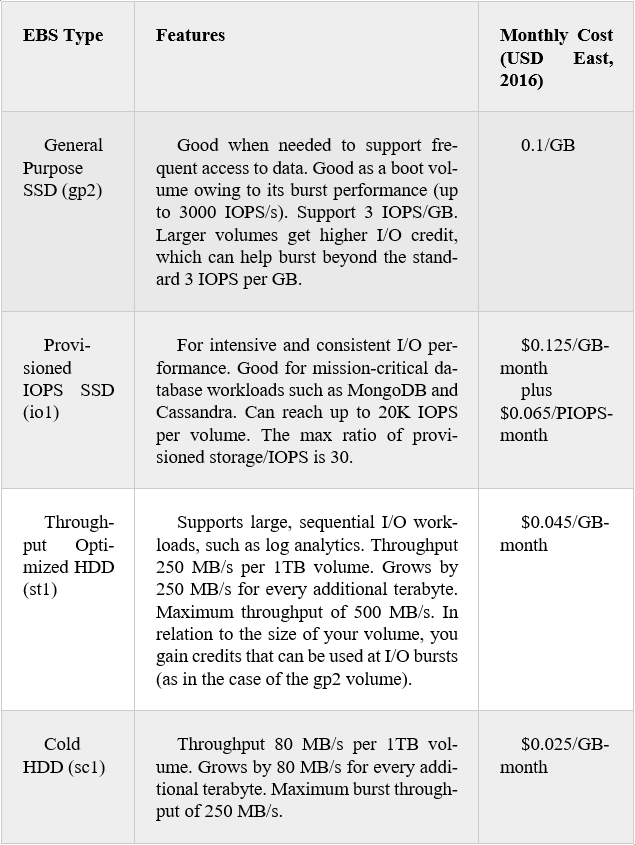
\includegraphics[width=10cm]{pic/ebs-pricing.png}
    \caption{EBS Pricing\cite{aws-ebs-pricing}}
    \label{EBS Pricing}
\end{figure}

\newpage
\section*{Appendix 3: S3 Pricing}
\addcontentsline{toc}{section}{Appendix 3: S3 Pricing}

\begin{figure}[H]
    \centering
    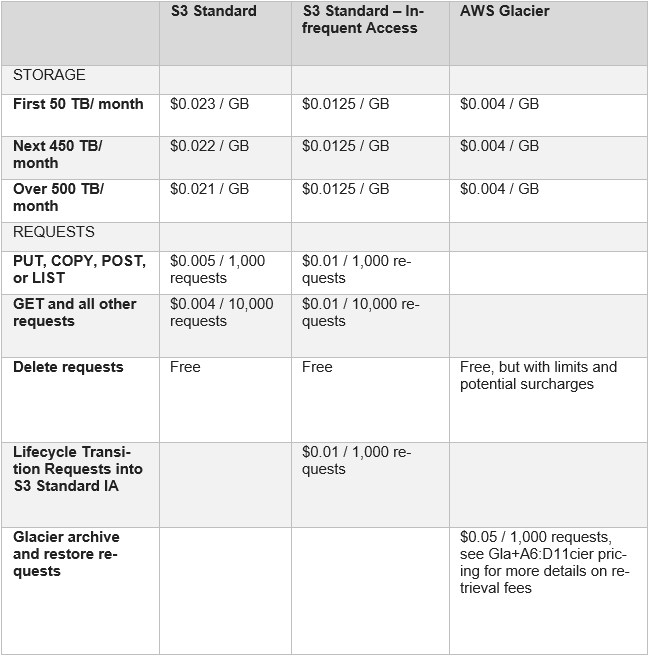
\includegraphics[width=10cm]{pic/S3-pricing.png}
    \caption{S3 Pricing\cite{aws-s3-costs}}
    \label{S3 Pricing}
\end{figure}

\end{document}